\documentclass[12pt]{article}

\setlength\parskip{0.4em}

\usepackage[utf8]{inputenc}
\usepackage[spanish]{babel}
\usepackage[T1]{fontenc}
\usepackage{newpxtext,newpxmath}
\usepackage{csquotes}
\usepackage{enumitem}
\usepackage{graphicx}
%\usepackage{epigraph}
%\usepackage{siunitx}
%\usepackage{graphicx}
\usepackage[dvipsnames]{xcolor}

\usepackage{hyperref}
\hypersetup{
	colorlinks=true,
	linkcolor=blue,
	filecolor=magenta,
	urlcolor=cyan,
}

\usepackage{caption}
%\captionsetup[figure]{labelformat=empty}

\title
{
	Escritos 2017-2021\\\vspace{0.5cm}
}

\author
{
	Jesús Gambín\\
	\normalsize{
		\texttt{\href{https://jdgambin.github.io}{jdgambin.com}}
	}
	\\\vspace{-1cm}
}

\date{}

\setcounter{secnumdepth}{0} 
\begin{document}
	\maketitle

	\begin{figure}[ht]
		\centering
		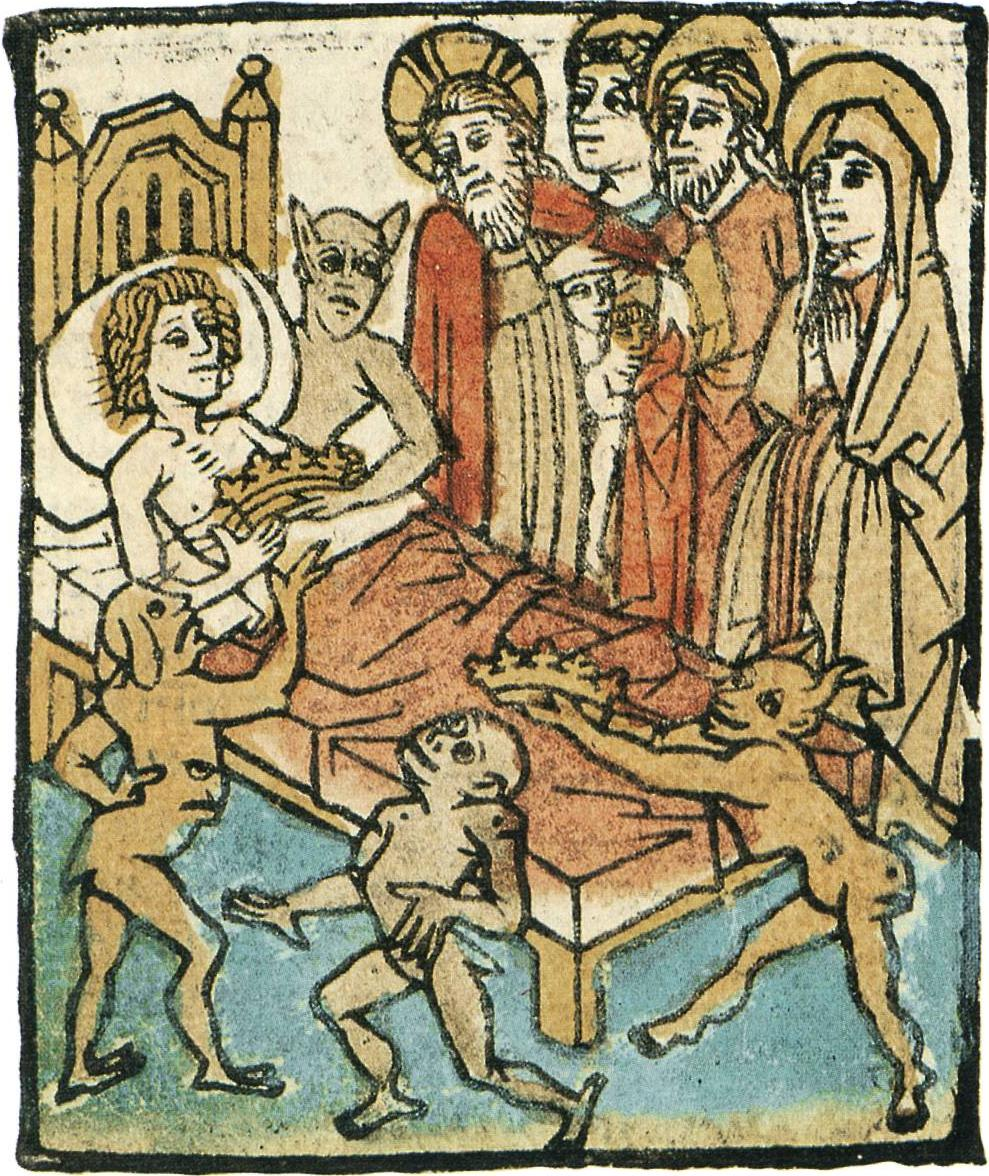
\includegraphics[scale=1]{portada}
	\end{figure}

	\vspace{0.8cm}

	\newpage

	\tableofcontents

	\newpage

	\section{2023}

	\subsection{Epígrafe}

	\textit{18 de julio de 2023}\\

	Estas cosas que escribí antes de mi conversión al catolicismo (en marzo
	de 2021) y poco después de la misma son de interés
	\textquote{biográfico} para mí, sobre todo, como he mencionado, son un
	referente en torno al acontecimiento de mi conversión a la fe católica a
	partir del ateísmo-agnóstico, materialista y hedonista, que sufrí
	durante más de una década antes de dar los primeros pasos en la
	dirección opuesta. Ciertamente, aunque caí muy bajo, no todo fue
	oscuridad.

	Cuando llegué a Dios todavía conservaba muchas inclinaciones malas y
	excéntricas de mi antiguo pensamiento y conducta que quedan plasmadas en
	estas páginas.

	Solo quiero decir antes de terminar esta introducción que la mejor
	manera de entender la mentalidad católica es viviendo con católicos de
	recta doctrina y costumbres, obedeciendo al Papa y a las autoridades
	respectivas dentro de la Iglesia, escuchando a buenos obispos y
	sacerdotes, que sean sabios y santos, leyendo la Sagrada Escritura, el
	Catecismo de la Iglesia Católica, los documentos del Magisterio
	eclesiástico y los libros católicos clásicos y tradicionales, leyendo 
	los escritos
	de los santos y conociendo las vidas de los santos y la
	\textit{verdadera} historia de la Iglesia.

	Doy aviso de que muchas de las aseveraciones concretas sobre filosofía o
	de ciencia relativa a las cosas sagradas que dejo por escrito en estos
	textos no son tan acertadas viniendo de un nuevo converso, pero el
	espíritu general de los textos no está tan mal, así que me permito
	publicarlos con algunas notas correctivas que puse en algunos
	escritos.\newline

	El primer escrito es un cuento corto, los demás son artículos de no
	ficción, entradas de \textquote{diarios}, varios de ellos, especialmente
	los últimos, son transcripciones de mensajes de voz que envié a amigos y
	así todos tienen orígenes y fines diversos.

	\newpage

	\section{2017}

	\subsection{El sueño de un hombre sensato}

	\textit{30 de abril de 2017}

	\blockquote[Ryūichi Kazama, \textit{Ping Pong the Animation}]
	{
		Todas mis células están cantando de alegría, me están ordenando
		que me mueva más rápido: \textquote{¡Más rápido! ¡Más rápido!}.
		Mi concentración bloquea el mundo exterior, nos estamos moviendo
		tan rápido que se siente como si el mundo estuviera detenido.
		Madura a una velocidad vertiginosa como si fuera normal, un
		cuerpo explosivo. Poco a poco se adelanta y siento
		que me va dejando atrás. Está claro quién es superior, pero no
		me siento ansioso. Estoy golpeando con todo lo que tengo, estoy
		reaccionando con todo mi ser. No tengo tiempo para estar
		asustado.
	}

	Sentado a la mesa del comedor del pequeño apartamento donde él y su
	familia residían, Calixto Herrán le comentaba a su hermana mayor los
	seductores efectos de una clase especial de fármacos, los
	estimulantes del sistema nervioso central. Sol, su hermana, estaba
	a punto de salir y atendía intermitentemente a Calixto, mirándose
	al espejo y arreglando uno que otro detalle antes de partir.

	--- Te hablaré en específico del \textit{Aderall} porque he leído
	testimonios de personas que lo han consumido por primera vez, después de
	haber presentado síntomas de TDAH en el pasado.

	--- ¿TDAH? ---interrogó la hermana, curiosa.

	--- ¡Oh!, significa \textquote{trastorno por déficit de atención e
	hiperactividad}. Seguro te suena, ¿no? Las personas que padecen TDAH
	tienen problemas para concentrarse y controlar sus impulsos. Las
	implicaciones son profundas porque afecta aspectos básicos de la vida
	\textquote{moderna} del individuo, en especial dentro del entorno
	académico y laboral.

	--- Ya había oído sobre eso, parece más severo de lo que imaginé.

	--- Pues, según entiendo, la condición solo genera problemas en
	instancias específicas. Los síntomas se manifiestan principalmente al
	realizar actividades que requieren de esfuerzo prolongado y que a su vez
	no son del todo placenteras o interesantes para el sujeto en ese
	momento. Es como tener el \textquote{músculo de la disciplina}
	debilitado.

	--- ¿Y a ellos les recetan los estimulantes como medicina?

	--- Sí... pero regresando a lo que quería decirte, muchas personas con
	problemas de atención son atraídas por estas sustancias. No es raro
	que algunos después de probar el Aderall por primera vez hagan
	declaraciones como \textquote{nunca me he sentido tan calmado y en
	control de mí mismo}, \textquote{realmente puedo escoger qué hacer en
	cualquier instante de tiempo}, \textquote{¿de esta manera se siente la
	gente normal?}, etc.

	--- ¿Tú quieres probar? ---dijo Sol, sonriendo momentáneamente.

	--- No realmente, la sensación eufórica por la que atraviesan y que
	tiñe su visión color de rosa no es permanente y desaparece a medida que
	su cuerpo se adapta a la droga. Las personas normales no experimentan el
	mundo como lo hacen ellos cuando sus primeras dosis surten efecto. De
	cualquier forma, lo que me interesa es el contraste y la sensación de
	libertad, algo paradójica, causada por la focalización ininterrumpida de
	la atención en las tareas a mano, sin mencionar los beneficios que este
	tipo de \textquote{devoción} trae consigo. Porque todos nos sentimos
	libres al dirigir nuestra fuerza de voluntad puntualmente hacia los
	objetivos que queremos alcanzar, ¿o me equivoco?

	Ambos permanecieron en silencio durante unos segundos hasta que Sol
	recogió su bolso, se despidió y se fue. Calixto fantaseaba con formas
	alternativas de alcanzar estados de consciencia similares ---pero más
	humildes--- a los descritos por los usuarios de estimulantes. Sol no
	compartía los mismos intereses que él, y por eso le habló a ella al
	respecto, para llamar su atención. No podía ser el único en la familia
	con tales inclinaciones, se decía a sí mismo de vez en cuando.

	Calixto se encontraba ahora acompañado únicamente de su libro de
	arquitectura minimalista, el cual había comprado con sus ahorros y que
	además estaba usando de momento para prepararse para una de sus
	clases, donde tenía que explicar su estilo favorito de diseño de
	exteriores. Con su presentación medio terminada y el libro abierto
	salió de su casa para caminar, relajarse y también pensar un poco.

	Dedicación a lo esencial, una razón para despertar al día siguiente, y
	para irse a dormir inquieto como un niño que sabe que conocerá el mar
	por primera vez al siguiente día después de haberlo visto pocas veces,
	pero con gran curiosidad, en fotografías o televisión. Calixto buscaba
	la manera más simple de crearse estas cosas para sí mismo. Mientras
	caminaba en la calle, miraba a su alrededor, a la gente, percibía los
	olores de la ciudad, los describía e indicaba sus orígenes, era como una
	afición intima, y en los últimos tiempos algo casi automático que hacía
	para pasar el rato mientras su cuerpo se distendía, se ejercitaba y
	salia de la monotonía de la silla. Las adicciones al entretenimiento
	y a las actividades pasivas que arrasaban con su tiempo sin dejar
	beneficio tangible alguno, pensaba él, habían ensombrecido lo mejor
	de sí e inhibido su desarrollo personal hasta un punto inaceptable.
	Todos sabemos cuales son en nuestra vida estas actividades fútiles,
	por tanto, no haré menciones particulares. Calixto regresó a su casa,
	su madre ya estaba allí, él la saludó y le preguntó cómo estuvo su
	visita al médico. Luego regresó a su silla y a sus libros, y se habló
	así:

	\blockquote[]
	{Una vez más es una vez menos, cada error puede acercarte más al
	terreno anhelado, sé ingenioso y piensa el cambio, prueba el cambio y
	decídete: vivir tu vida con intención, ese es el sueño de un hombre
	sensato.}

	\begin{center}FIN\end{center}

	\newpage

	\section{2019}

	\subsection{Sobre el uso de las computadoras e Internet}

	\textit{13 de noviembre de 2019 --- escrito originalmente en inglés}

	\subsubsection*{Introducción}

	Nuestros cerebros han sido moldeados por hábitos dañinos de Internet y
	por años de refuerzo. La única solución es eliminar todo rastro de
	distracción y suciedad de nuestra vida diaria. Mi nuevo objetivo es
	dejar de navegar por la web y usarla solo para cosas verdaderamente
	esenciales que sirvan a mis valores más importantes.

	La Web se ha convertido en un agujero negro de atención donde millones
	de personas trabajan constantemente para engañar a nuestros cerebros y
	robar nuestra preciada atención en detrimento de nuestras capacidades
	mentales y nuestra independencia. De hecho, tales fuerzas quieren que
	nos transformemos en una especie de sirvientes zombis. Esto no es una
	broma, es la realidad. No puedo enfatizar cuán serio creo que es este
	problema.

	Abogo por el \textquote{extremismo}. Lo pongo entre comillas porque
	puede parecer extremismo para nosotros que hemos abusado de la
	tecnología, pero de hecho, abogo por un estado más congruente con
	nuestra naturaleza humana esencial y \textit{constante}.

	¿Qué significa esto en la práctica? Dejar de usar cualquier tecnología
	digital que realmente no necesites y usar siempre la tecnología de forma
	controlada.

	El \textquote{minimalismo digital}, la filosofía del uso de la
	tecnología descrita por Cal Newport en su libro \textit{Minimalismo
	digital} es el futuro. Eso es en lo que creo.

	Espero que tengamos la fuerza para cambiar y estar más enfocados en lo
	que queremos hacer con nuestras vidas, y usar eso como motivación para
	dejar los hábitos dañinos. Este es el mejor consejo que puedo dar, y es
	muy difícil de seguir en nuestras condiciones actuales. El propósito
	general de todos los seres vivos es resolver sus problemas. La
	resolución de problemas es el sentido de la vida. Maximiza tus recursos
	para ello.

	Necesitamos construir hábitos y motivaciones fuertes para
	\textquote{sobrescribir} los hábitos creados por las adicciones. Estoy
	tratando de concentrarme mucho en los campos de estudio que amo. Quiero
	aprender mucho. La adicción a las cosas relacionadas con Internet es tan
	dañina para nuestras mentes e inteligencias que no puedo ver cómo podemos
	cambiar una vida rica por estos placeres pequeños y sin sentido que
	cualquier bestia puede explotar.

	\subsubsection*{Por qué y cómo}

	¿Por qué no puedo ceder? Simple: Mi cerebro está adaptado a muchos
	hábitos dañinos.

	\begin{enumerate}
	\item Si cedo, fácilmente renovaré mi fase adictiva una vez más (porque
		mi cerebro está muy adaptado a los malos comportamientos).
	\item Si entro en un nuevo período de comportamiento adictivo
	compulsivo, estoy reduciendo gran parte del potencial de mi cerebro para
	la función cognitiva inteligente (porque estas adicciones que tengo me
	hacen más estúpido, literalmente).
	\item Si reduzco el potencial de mi cerebro para la función cognitiva
	inteligente, entonces no podré resolver mejor mis problemas en la vida y
	atrofiaré mi comprensión de mí mismo, de las cosas específicas que amo y
	del mundo en general; limitando así mi vida en un grado enorme, y no
	dejaré que eso suceda. No tienes idea de lo importante que es esto para
	mí.
	\end{enumerate}

	Básicamente, en términos muy generales, mis principales motivadores
	contra los malos hábitos son

	\begin{itemize}
	\item Quiero ser cada vez más y más inteligente.
	\item[] \textit{lo que da apoyo para...}
	\item Quiero entender más sobre las cosas que me interesan.
	\item[] \textit{lo que da apoyo para...}
	\item Quiero tener éxito en la aplicación de mis conocimientos y
		habilidades para dar solución a todo tipo de problemas.
	\end{itemize}

	Cuando tenemos tentaciones de todo tipo necesitamos observar nuestro
	ser con un enfoque detallado y tomar la decisión correcta de ignorar las
	malas inclinaciones y calmarlas porque ahora estamos en un camino
	diferente. Estamos luchando por nuestra libertad, amigos.

	Hoy tengo un antojo de algo dañino. ¿Qué debo hacer?

	\begin{enumerate}
	\item Aceptar con calma que tengo un deseo vicioso.
	\item Tratar de buscar una razón. Si hay una razón clara por la cual me
		encuentro tentado, recordarla
	para no caer en la trampa otra vez.
	\item No reaccionar ante ello. Concentrar la atención en otra cosa.
	\item Cambiar de escenario, buscar un entorno menos nocivo.
	\end{enumerate}

	\subsubsection*{Compromisos}

	Vuelvo a intentar librarme de estos hábitos nocivos después de fracasar
	con intentos desestructurados y vagos deseos. Quiero intentar
	abstenerme básicamente de todos los medios modernos:

	\begin{itemize}
	\item Navegación web, incluidas todas las redes sociales (excepto foros
	de Internet útiles con una función específica).
	\item Películas, series de TV, anime, documentales y servicios de
	streaming de video (YouTube, Netflix, Twitch, etc.).
	\item Música.
	\end{itemize}

	Estas cosas han estado con nosotros durante casi tanto tiempo como hemos
	podido respirar. Hoy en día, tenemos una tolerancia muy baja para el
	aburrimiento y la soledad. Quiero una mente más pura y poderosa. Una
	mente mejor sería capaz de crear una mejor calidad de vida para ti y
	para las personas que te rodean. Eso es lo que pienso.

	Eliminé todas mis cuentas de redes sociales hace mucho tiempo. Ya no
	juego videojuegos, y no planeo comenzar a jugarlos nunca más. Es por
	eso que no los agregué a la lista, las cosas enumeradas allí son mis
	últimos vicios (que yo sepa) y los voy a aplastar lenta pero
	inevitablemente.

	Registraré todas las excepciones que haga a este estilo de vida durante
	mi día (como soy estudiante universitario, a veces necesito ver algunos
	videos para extraer información valiosa), ninguna de estas excepciones
	puede tener como único o principal objeto el consumo de los medios por
	entretenimiento (ya sea un video tutorial, documental, entrevista, etc.).
	Todo es con fines educativos y productivos y lo justificaré
	explícitamente cuando sea necesario.

	Acerca de mi historial de navegación web: básicamente lo registraré
	todo, a diario, y lo haré público para ayudarme con esto. Finalmente le
	daré un buen uso a mi historial de navegación.

	¿Por qué hago todas estas cosas? Es un experimento muy importante sobre
	la naturaleza de mi experiencia cognitiva. Este es el mejor estilo de
	vida para preservar dopamina.

	\subsubsection*{Ejemplo: Cómo dejé los videojuegos}

	¿Qué tan difícil es dejar los videojuegos para siempre? Fue muy difícil
	para mí. Hice esto:

	\begin{itemize}
	\item Eliminé todos mis videojuegos del disco duro y deseché todas mis
	cuentas de servicio de videojuegos (Xfire, Steam, etc.).
	\item Les dije a todos mis amigos que dejaría los videojuegos y rechacé
	todas las invitaciones para jugar.
	\item Concentré mi energía en actividades productivas que valoraba en
	ese momento (educación, matemáticas, computación, programación de
	computadoras, etc.).
	\end{itemize}

	Eso fue todo lo que hice. Me llevó algunos meses dejarlo todo
	definitivamente, pero al final funcionó bastante bien (dejé todo desde
	el 2014). Ya no soy adicto a los videojuegos. Son una pérdida de
	tiempo para mí.

	También me estoy deshaciendo de la música, las series de televisión, el
	anime y las películas. Sí, leíste eso bien. Ya eliminé todo eso de todos
	mis dispositivos. Me encanta este tipo de pureza.

	He dedicado una cantidad inmensa de horas a estas cosas, ahora quiero
	enfocarme en ser más activo. Recomiendo encarecidamente practicar
	deportes, no hice esto en el momento en que dejé los videojuegos, pero
	me habría ayudado inmensamente. Elegí artes marciales (Taekwondo y MMA,
	mi estilo favorito es el kickboxing holandés).

	\newpage

	\section{2020}

	\subsection{Propuesta de tesis de pregrado en bioinformática}

	\textit{17 de febrero de 2020}\\

	En primer lugar quiero agradecerles su interés en mi intención de
	elaborar una tesis de pregrado relacionada con la bioinformática y por
	la amabilidad de considerar lo que tengo que expresar. Mi nombre es
	Jesús Gambín y soy estudiante de Ingeniería de Sistemas [1]. La
	decisión de incursionar en esta dirección es reciente, y me encuentro
	investigando parte de la literatura existente en busca de contenido que
	integre las nociones y habilidades básicas que he adquirido en mi
	educación.

	Las principales ideas que he examinado son:

	\begin{itemize}
	\item
		\textit{Biología ejecutable} y modelos computacionales para el
		modelado algorítmico y discreto de sistemas biológicos [2][3].
	\item
		\textit{Modelos matemáticos} para representar aspectos
		biológicos como relaciones entre cantidades matemáticas
		continuas [4][5].
	\item
		\textit{Aprendizaje automático} para el modelado predictivo o
		extracción de información de interés en función de grandes
		bases de datos biológicas y algoritmos de aprendizaje [6][7].
	\item
		\textit{Organismos digitales} para la simulación y estudio de
		dinámicas evolutivas [8][9].
	\end{itemize}

	Mi plan actual, muy general, para una tesis de pregrado en relación a
	estos temas consiste en una colección de \textquote{modelos biológicos}
	implementados por software. La ejecución consta de tres grandes pasos:

	\begin{enumerate}
	\item
		Investigar y entender un modelo particular o seleccionar una
		base de datos tratable por medio del aprendizaje automático.
	\item
		Obtener un algoritmo que aplique el modelo para implementarlo
		como programa de computadora.
	\item
		Una vez alcanzada una masa crítica de ejemplos de modelos,
		refinar el trabajo, su documentación y finalizar la preparación
		de la tesis para su presentación.
	\end{enumerate}

	Mi objetivo es mostrar los principios que incrementarán el poder
	predictivo de la biología como ciencia natural y que conducirán a la
	aceleración del avance de sus aplicaciones. En acuerdo, y motivado por
	las generalizadas ideas que manifiesta la siguiente cita:

	\blockquote
	[Alejandro B. Engel, Elementos de Biomatemática, 1978]
	{\textit{La meta básica de la ciencia moderna es crear, en torno a los
	fenómenos reales, modelos que describan y puedan predecir el
	comportamiento de tales fenómenos.}

	\textit{[...]}

	\textit{Probablemente debido a nuestra limitación intelectual, es claro
	hasta cierto punto que el porqué de las cosas nunca tendrá una
	respuesta, a no ser una basada en otros hechos cuyo porqué será un nuevo
	enigma. Sin embargo, la experiencia nos muestra que, si no podemos
	comprender, al menos podemos predecir, dentro de ciertas limitaciones,
	cómo suceden los fenómenos naturales.}}

	Mis puntos fuertes:

	Leo, escribo, y entiendo inglés sin problemas (B1 CFER en 2013,
	certificado por ICFES). Puedo aprovechar el material técnico e informal
	en inglés de libros, artículos, conferencias y entrevistas
	videograbadas, etc. Tengo familiaridad con los sistemas formales, la
	lógica y las pruebas matemáticas [9]. También manejo los conceptos
	básicos del cálculo y puedo aprender teoría matemática de modo
	independiente. Programo de manera recreativa desde el bachillerato y he
	usado una variedad de lenguajes de programación imperativos como C, C++,
	Java, C\#, Python, Bourne Shell (en Linux), etc. Estoy dispuesto a
	estudiar conocimiento de fondo (biología, química, etc.) y tengo un
	firme interés en las ciencias naturales y formales así como en su
	intersección productiva con la informática y la computación. También
	cuento con una decente biblioteca en mi universidad, con buena cobertura
	de temas científicos y tengo destreza en la búsqueda de literatura
	electrónica en internet.

	Mis puntos débiles (que estoy trabajando en fortalecer):

	Cuento con muy poco conocimiento en los ámbitos de biología y química.
	No he desarrollado \textquote{software científico} ni de simulación en
	el pasado. Tampoco he realizado proyectos de modelado predictivo con
	base en técnicas de aprendizaje automático. Estoy abierto a cualquier
	sugerencia sobre mi dirección por parte suya, cuya experiencia
	valoro ampliamente dado que una de mis expectativas es la posible
	incursión a largo plazo en el campo de la bioinformática (como
	investigador o desarrollador de aplicaciones en áreas de alto impacto
	social como la medicina o la agricultura) y cualquier progreso en este
	sentido lo aprecio de verdad. Por tanto, quiero explicitar que, en caso
	de que decidan apoyarme significativamente a lo largo del desarrollo de
	mi tesis e independientemente de mis intereses actuales en la materia,
	estoy dispuesto a trabajar en lo que consideren adecuado y relevante a
	su área de conocimiento. También quiero señalar que no trabajo bajo
	exigencias estrictas de tiempo, pues cuento con al menos dos años y
	medio para culminar el trabajo.

	Muchas gracias por su atención.

	\subsubsection*{Referencias}

	\begin{enumerate}[label={[\arabic*]}]
%	\setcounter{enumi}{-1}
	\item Adjunto un certificado académico.
	\item \textit{Executable cell biology} (J. Fisher, et al.).
	\item \textit{Computational Modeling, Formal Analysis, and Tools for
		Systems Biology} (E. Bartocci, et al.).
	\item \textit{Mathematical Biology I: An Introduction} (J. D. Murray).
	\item \textit{Mathematical models in biology. An introduction}
		(E. S. Allman).
	\item \textit{Deep learning for computational biology}
		(C. Angermueller, et al.).
	\item \textit{Machine learning in bioinformatics} (Wikipedia:
	\url{https://en.wikipedia.org/wiki/Machine_learning_in_bioinformatics}).
\item \textit{About Digital Evolution} (Avida Wiki:\ 
	\url{https://github.com/devosoft/avida/wiki/About}).
	\item \textit{Avida: A Software Platform for Research in Computational
		Evolutionary Biology} (C. Ofria, et al).
	\item En particular, aprobé el primer curso semestral de introducción a
		las demostraciones matemáticas ofrecido a los estudiantes del
		programa de Matemáticas de mi universidad.
	\end{enumerate}

	\newpage

	\subsection{La superficialidad de la cosmovisión predominante}
	\setcounter{footnote}{0}

	\textit{3 de mayo de 2020 --- escrito originalmente en inglés}\\

	¿Estás en un mal estado de ánimo? ¿O crees que tu principal problema es
	haber descubierto la sombría y dura \textquote{verdad} sobre el mundo?
	Este es el resultado de haber asimilado como verdad las filosofías y
	puntos de vista expresados en la cultura hipersecular, materialista y
	atea que prevalece en la sociedad actual. Esto es muy tóxico y dañino.

	Primero, date cuenta de que el mundo es más que su apariencia exterior.
	Esto es de conocimiento común y está confirmado por la ciencia, siendo
	el ejemplo usual el espectro visible, pero este es solo uno de infinitos
	ejemplos. Entonces, pase lo que pase, las cosas no pueden ser
	\textit{simplemente} lo que parecen ser. No seas ingenuo con frases del
	tipo \textquote{¡equis cosa material lo es todo en la vida!}. Eso no
	tiene ningún sentido. Puedes tener una \textit{buena} vida incluso si no
	tienes (según el mundo) éxito económico, social o sexual.

	Ahora, recuerda que hay valores superiores como la verdad, la belleza,
	la bondad, etc. que realmente pueden guiarte en tu vida y brindarte una
	conciencia limpia. Cualquier ser humano suficientemente desarrollado con
	sentido de la realidad sabe que estas cosas son reales. Ten eso en
	mente.

	Hacer lo correcto es difícil, por ejemplo, decir la verdad o reconocer
	una verdad que no te conviene. Pero esforzarse por ser bueno y honesto
	te dará la tranquilidad que afanarse por acumular bienes materiales (o
	creer cualquier otra tontería salida de los medios de comunicación
	de masas) no puede dar.

	Si estás deprimido por ser un \textquote{nihilista} es porque te falta
	paz (no es porque no puedas conseguir un placer particular ahora o más
	tarde o cuando sea). Hay un conflicto con la realidad. Si estás leyendo
	esto y estás deprimido, probablemente estés desesperado por algo,
	podría ser tu \textquote{vida romántica}, tu apariencia física o
	cualquier otra cosa que sea igualmente mundana. No importa.

	Te insto a que empieces a educarte en asuntos espirituales (en general,
	tendrás que tomarte muy en serio toda tu educación). Una cosa que me ha
	ayudado mucho es investigar el reservorio de sabiduría religiosa
	sintetizada por los pensadores modernos (solía descartar todo lo
	relacionado con la religión como superstición mística, pensé que yo era
	demasiado racional para eso, fue un error). Si estás interesado en esto,
	puedes comenzar leyendo autores como C. S. Lewis (sus obras de no
	ficción como \textit{Mere Christianity}, \textit{The Abolition of Man},
	\textit{The Screwtape Letters}, etc.) o \textcolor{red}{Aldous Huxley
	(\textit{Filosofía perenne}, sus artículos y sus obras de ficción
	como \textit{Brave New World} e \textit{Island})}.


	Algunos ejemplos de lo que quiero decir:

	\begin{itemize}

	\item \textit{Evangelio de Mateo 7,13-21}:
	estos son conceptos contundentes, vivir de acuerdo con ellos requiere
	que no te engañes y tengas una actitud rigurosa con respecto a tu
	comportamiento.

	\item \textcolor{red}{\textit{Vedanta for the Western World}: esta
	es una compilación de artículos de la revista del mismo nombre. Es una
	explicación moderna de los puntos fundamentales de la religión,
	podría considerarse como un estudio de la religión universal (este es un
	legado de la sabiduría humana sobre cómo vivir, cómo ver el mundo y cómo
	encontrar la verdad). Recomiendo comenzar leyendo los artículos de
	Aldous Huxley (es decir, \textit{The Minimum Working Hypothesis},
	\textit{Distractions I} y \textit{Distractions II}, etc.)
	\footnote{\textcolor{red}{
		\textit{Nota de 2023}: Actualmente y desde 2021 desapruebo leer
			los artículos
	religiosos de
	Aldous Huxley y de corrientes asociadas o similares como fuentes
	fiables de verdad, pues contienen errores fatales. La única autoridad
	conferida por Jesucristo en términos religiosos es la Iglesia
	Católica, los demás \textquote{maestros} están en absoluta oposición o
	como mínimo, separados de Ella en grados de mayor o menor error.
	\textit{Brave New World} sigue siendo una lectura interesante porque
	muestra las aberraciones de la mentalidad moderna.}}.}
	\end{itemize}

	Hay mucho material, pero puedes comenzar con estos recursos o puedes
	buscar otros por tu cuenta. Estás equipado para encontrar la verdad, el
	problema es que no tenemos buenos guías. La televisión y las redes
	sociales envenenarán tu mente, pero se puede cambiar, yo soy prueba de
	ello.

	Si la sociedad estuviera organizada de una buena manera con una buena
	cultura, entonces los rincones del mundo con personas deprimidas
	obsesionadas con cosas superficiales como la cirugía plástica, el dinero
	y dominar a los demás, ni siquiera existirían. Este no es el caso, así
	que tienes que educarte para alcanzar las verdades que, en nuestro
	estado actual, no te serán enseñadas naturalmente.

	\newpage

	\subsection{¿El \textquote{progreso} fue un error?}

	\textit{28 de julio de 2020}

	\begin{displayquote}
	[Nicolás Gómez Dávila, Escolios a un texto implícito: Tomo II, n. 102.]
	\textit{El mundo moderno nos exige que aprobemos lo que ni siquiera
	debería atreverse a pedir que toleráramos.}
	\end{displayquote}

	A continuación citaré varios extractos de los artículos
	\textquote{Los niños transgénero que retrasan su pubertad para tener más
	tiempo para decidir sobre su sexo}\footnote{\url
	{https://www.bbc.com/mundo/noticias-america-latina-44355521}}
	y \textquote{Muchos niños y niñas trans no llegan a los 14 años, se
	suicidan, o llegan ya con mucho daño en su salud}\footnote{\url
	{https://www.bbc.com/mundo/noticias-44684416}} ambos publicados por
	\textit{BBC News Mundo} (dentro de las citas escribiré mis propios
	pensamientos dentro de corchetes en la siguiente forma
	\textquote{\textbf{[\texttt{JG}: ...]}}):

	\begin{displayquote}
	\textit{\textquote{Estoy contenta de que me hayan dado la medicación
	porque ahora sé que no me va a salir vello facial. No quiero barba, soy
	una chica}. Son palabras de Jessica, de 11 años y una de los más de 300
	niños transgénero que cada año toman tratamiento para
	bloquear la llegada de la pubertad en Reino Unido.}

	\textit{[...]}

	\textit{Lily, otra niña británica transexual que habló con la BBC, tiene
	10 años y ya ha tenido que lidiar con comentarios intrusivos en
	su escuela primaria.}

	\textit{[...]}

	\textit{Esta medicación, que se le ofrece desde 2011 a los menores de
	16 años, es una manera de \textquote{comprar tiempo} para que puedan
	pensar y decidir con menos presión cómo quieren vivir sus
	vidas.}

	\textit{[...]}

	\textit{\textquote{Muchos niños y niñas trans no llegan a los 14 años,
	se suicidan, o llegan ya con mucho daño en su salud mental}, describe
	Mónica.}

	\textit{[...]}

	\textit{Aunque su partida de nacimiento decía que era un niño, ya a
	los 2 años su hija transexual había empezado a manifestar una
	identidad de género distinta.} \textbf{[\texttt{JG:} esto afirma Mónica
	sobre su propio \textit{hijo}.].}

	\textit{[...]}

	\textit{\textquote{Nosotros creemos que la identidad de género es un
	derecho humano y que, segundo, no es una decisión, por lo tanto no hay
	una edad para prohibirlo o autorizarlo. Tenemos testimonios de niños de
	5, 6, 7, 8, 9 años que han hecho su tránsito y viven su identidad de
	género. Entonces por qué no tener ellos el derecho a ser reconocidos en
	su país.}} \textbf{[\texttt{JG:} palabras de Mónica, madre de un hijo
	abusado.]}.

	\textit{[...]}

	\textit{La hija de Mónica Flores tiene 7 años. \textquote{Hasta ahora
	está protegida, tras los primeros años, que fueron dolorosos, hemos
	aprendidos juntos, nos hemos acompañado como familia}.}
	\end{displayquote}

	¿Qué te parece? Aquí otra historia \textit{real}: Anne Georgulas y
	Jeffrey Younger son padres de un hijo varón. La madre, Anne, una
	pediatra, quería que su hijo \textquote{cambiara de sexo} y esta idea no
	le gustó al padre, así que fueron a la corte para tomar una decisión
	respecto al \textquote{asunto}. ¿Adivinas el resultado?

	\blockquote[]
	{\textit{Un jurado popular falló excepcionalmente a favor de la
	madre por 11 votos a favor y sólo uno en contra.}

	\textit{Tras escuchar a los padres, maestros y terapeutas, un jurado
	popular de Dallas falló a favor de la madre por 11 votos a favor
	y sólo uno en contra, un resultado excepcional en este tipo de
	casos en los que lo habitual es inclinarse por el padre que
	defiende el sexo biológico del menor. En medio de una gran
	presión social, horas después, la juez del tribunal familiar que
	lleva el caso, Kim Cooks, decidió desoír el veredicto y ordenó a
	los padres compartir la custodia.}}

	No es un sueño, este es nuestro mundo y va a empeorar. Esto es solo un
	ejemplo del tipo de degeneración que existe, no es algo aislado, y es
	tan solo una de las manifestaciones del absurdo espíritu de nuestro
	tiempo. Uno debe ser capaz de observar esto y reconocer que algo está
	muy mal con el mundo de hoy, en donde, entre otras cosas, estas
	atrocidades son defendidas por la cultura e ideologías en ascenso. De
	estos hechos podemos aprender mucho, porque si uno no es consciente aún,
	las raíces de las peores influencias sociales pueden ser descubiertas
	partiendo de la observación de los actos abominables de ciertos
	individuos que quieren, y están logrando con éxito, obtener una
	creciente protección e integración de sus valores destructivos en
	nuestras vidas cotidianas y en la estructura esencial del sistema
	social, y gozan de una creciente popularidad y aprobación por parte de
	las masas.

	Esta inversión de los valores tradicionales, aquellos que hemos depurado
	durante milenios y que nos han hecho sobrevivir, debe ser repudiada,
	puesto que su principal producto es la miseria y el deterioro
	humano, de los ecosistemas terrestres y de básicamente todo lo bueno,
	hermoso y verdadero.

	\begin{displayquote}
	[Nicolás Gómez Dávila, Nuevos escolios a un texto implícito]
	\textit{Las mayorías de una sociedad tienen determinada mentalidad
	porque la sociedad tiene determinada estructura, pero la sociedad tiene
	determinada estructura porque una minoría tiene determinada mentalidad.}
	\end{displayquote}

	Existe una elite que promueve valores destructivos y la mayoría de
	nosotros los aceptamos acríticamente. La gente es controlada y
	minada mediante sus vicios. ¿Qué promueve Hollywood o la industria
	de la música \textit{mainstream} occidental? Colombia todavía no está
	en el nivel de perversidad de Europa Occidental o de América del Norte,
	pero esa es la dirección del mundo: El hombre promedio y la mujer
	promedio contemporáneos son un receptáculo de la peor cultura que ha
	existido en la historia y se les alimenta con eficiencia, pues tenemos
	la tecnología para hacerlo. Y me he limitado a hablar un poco de la
	destrucción del humano, pero los valores modernos también implican
	destrucción del medio ambiente. Por ejemplo, el consumismo o la
	industrialización y la urbanización en exceso.

	Estudiar el desarrollo de la cultura es necesario para entender nuestra
	situación actual y parar de pensar ingenuamente que vivimos en
	\textquote{el mejor de los mundos} o que somos la civilización
	\textquote{más avanzada} que ha existido, etc. Al parecer los antiguos
	nos superaban en cosas más importantes que el progreso tecnológico y
	económico. Pero nos damos por superiores e imparables, y hasta dioses,
	porque actualmente a los valores materiales se les confiere mayor
	importancia y se dejan las virtudes y los temas espirituales de lado.
	Esto es un error, puesto que como es fácil de observar: \textquote{el
	hombre no vive solo de pan}, piensa en esto.

	A menudo pienso en las acusaciones contra el hombre moderno que lo
	describen como la epítome de la mediocridad humana (cómodo,
	autocomplaciente, idiotizado por la especialización y la domesticación 
	que los vuelve literalmente engranajes intercambiables de la maquina y
	poco más que \textit{NPC's} conectados a la \textit{matrix} del complejo
	industrial de entretenimiento y de los vicios, esclavos asalariados
	contentos, etc.) y no es difícil creerlo. Pero la mentalidad humana no
	ha sido siempre así, esto hay que entenderlo.

	Veo que nos definen cosas como la visión de túnel materialista, el
	cientificismo, y otras creencias estúpidas como el generalizado supuesto
	del \textquote{progreso} constante como destino natural de la historia,
	el hedonismo que nos aleja de la búsqueda de valores elevados y nos roba
	nuestra dignidad, y un largo etcétera.

	No llegamos a este punto solos, hay fuerzas que actúan y nos mueven en
	la dirección equivocada y todo humano consciente debe tomarse el trabajo
	de entender este proceso y de encontrar qué hacer para lograr llevar una
	vida como se debe y no como nos condiciona automáticamente nuestro
	entorno actual.

	En mi opinión, para alejarse del mal hay pasos prácticos que tomar que
	no discutiré aquí (por ejemplo, alejarse de las ciudades, comprar tu
	propia tierra y crear independencia o autosuficiencia). Pero quiero
	recomendar autores buenos que comprenden este fenómeno del que he
	escrito en los párrafos anteriores: Nassim Nicholas Taleb, del cual
	estoy leyendo \textquote{Jugarse la piel}, también su libro
	\textquote{Antifragil} parece muy bueno. Otro autor es el filósofo
	colombiano Nicolás Gómez Dávila, de este tengo los dos tomos de
	\textquote{Nuevos Escolios a un Texto Implícito}. Algo que me ha ayudado
	mucho a abrir los ojos es la novela de Aldous Huxley,
	\textquote{Un Mundo Feliz}, que refleja increíblemente bien la dirección
	que seguimos. Con respecto a esta novela, hay una situación cómica en la
	que me he encontrado, y es que entre más piensas como un
	\textquote{moderno} menos malo te parece el mundo del libro, yo he leído
	ese libro en varias etapas de mi vida, y me he fijado en esto. Creo que
	entre menos claro sea para alguien lo malo del nuevo mundo de esta
	novela, más reformación interna necesitará como persona.

	\newpage

	\section{2021}

	\subsection{Sobre la propuesta de bioinformática}

	\textit{Enero de 2021}\\

	\textquote{Propuesta de tesis de pregrado en bioinformática} fue el
	email que envié hace un año a unos biólogos (uno era especialista en
	bioinformática) con los que un amigo me había puesto en contacto, quería
	que me asistieran para hacer mi tesis de pregrado sobre algún tema de
	bioinformática. Quedamos en que yo iba a hablar con un profesor de mi
	departamento que trabaja en \textit{machine learning}, pero cuando se
	aplazaron las clases de la universidad por la pandemia de COVID-19 dejé
	de escribirles, porque al final ya no estaba seguro de siquiera querer
	hacer una tesis así.

	Lo que hice fue investigar cosas que integraran informática y biología,
	la más realista de todas fue la de \textquote{aprendizaje automático}
	porque se trabaja tomando bases de datos y software y no necesita de
	conocimiento específico de biología sino más que todo saber aplicar
	algoritmos sobre los datos para obtener resultados útiles (hay mucho
	más ensayo y error e ingeniería que \textquote{entendimiento} de la
	biología involucrada).

	En ese tiempo tuve una idea que me causó curiosidad, mi idea para la
	tesis era explorar los métodos que aprovechan la informática para hacer
	de la biología una \textquote{ciencia más precisa} como la física, que
	es el ideal moderno de la comunidad científica (donde solo importan los
	resultados de los modelos cuantitativos que \textquote{recrean} o
	\textquote{predicen} los datos empíricos). Esto lleva al segundo enfoque
	de mi lista que son los modelos matemáticos continuos, generalmente
	basados en cálculo y ecuaciones diferenciales, pero incluye otros tipos
	de matemáticas también (matemáticas \textquote{discretas} como la lógica,
	el álgebra abstracta, la teoría de conjuntos y los números enteros que
	se distinguen de las matemáticas \textquote{continuas} como el cálculo,
	el análisis y los números reales).

	Luego encontré el primer enfoque que listé en mi correo,
	\textquote{biología ejecutable}, que como los modelos matemáticos
	intenta predecir, pero su naturaleza es más cualitativa que
	cuantitativa, esta no utiliza matemáticas continuas sino algoritmos y
	procesos discretos para describir los fenómenos naturales. Esto se
	entiende mejor cuando tienes algo de experiencia en programación, la
	biología ejecutable trata de programas digitales que imitan procesos
	biológicos que se pueden conceptualizar como algoritmos (una serie
	ordenada de instrucciones para lograr un fin determinado). Estos
	algoritmos se implementan en computadoras para hacer simulaciones, y así
	\textquote{predecir}, de manera similar como en los modelos
	cuantitativos clásicos de la física; pero en vez de usar ecuaciones
	matemáticas, el medio para modelar son los programas de computadora.

	Me interesé en esto porque en informática hay herramientas
	potentes para el análisis de programas y la verificación de sus
	propiedades, por tanto, en principio, se podrían usar estas herramientas
	(disponibles para analizar software) pero ahora con la intención de
	analizar los modelos algorítmicos que representan los
	\textquote{sistemas biológicos reales} usando la lógica formal que se
	usa en informática para analizar los programas ordinarios. Si lo que
	digo no es entendible, es normal, estoy tratando de resumir lo que
	pensaba en ese tiempo, se entiende con mayor contexto y también cabe la
	posibilidad de que no este diciendo cosas coherentes (solo investigué
	estas cosas por un corto tiempo hace un año).

	Esta idea me sorprendió porque, suponiendo que tengas un modelo de este
	tipo que refleje la realidad de un proceso biológico, digamos, algún
	proceso fisiológico de un animal microscópico (y hay un ejemplo de esto
	en uno de los artículos que revisé, aunque el modelo es extremadamente
	complejo y no sé que tan efectivo sea) entonces analizar automáticamente
	las propiedades de un programa de computadora que modele el
	comportamiento biológico de este animal correspondería a, por
	ejemplo, analizar el crecimiento de uno de sus órganos o algo por el
	estilo, depende del propósito del modelo.

	Otra cosa que me interesaba era la aplicación de estos modelos en el
	nivel de descripción molecular, porque ya existen modelos precisos para
	los fenómenos que ocurren en este nivel contribuidos por la química y la
	física. Entonces, la \textquote{suma} de los modelos de la física y la
	química unidos al poder de aplicación de la informática convertiría a
	la biología en una ciencia natural más determinista, precisa, exacta,
	más parecida a la física; así pensaba yo. La informática era necesaria
	porque los datos de la biología son muy complejos, y ningún humano puede
	realizar el tipo de cálculos que nos importan acerca de los fenómenos
	biológicos de manera suficientemente detallada en su mente debido a que
	la cantidad de datos a considerar es masiva y complicada.

	Recapitulando: los primeros dos enfoques fueron (1) la biología
	ejecutable y (2) los modelos matemáticos en biología, ambas técnicas
	se relacionan con la implementación de modelos mediante computadora. Me
	causaban mucha curiosidad debido al potencial de combinarlos y
	aplicarlos a las descripciones de más bajo nivel de los procesos
	biológicos (susceptibles al tratamiento de los modelos cuantitativos de
	la física y la química) que supuestamente determinan los aspectos
	macroscópicos de la biología (materialismo reduccionista). Todas mis
	explicaciones aquí son simplistas, pero la idea general que tenía era
	que si combinabas la informática con el estudio de la biología en los
	niveles relevantes, entonces podrías convertir la biología en una
	ciencia exacta, o al menos existiría el potencial de acercarnos a este
	ideal tanto como fuese posible.

	Finalmente, están los últimos dos enfoques: (3) aprendizaje automático y
	(4) organismos digitales. Solo hablaré del último porque ya he escrito
	mucho y estoy aburrido. El último enfoque de mi lista trata de estudiar
	la evolución mediante la formalización de las reglas y conceptos del
	pensamiento evolutivo (aptitud, replicación, mutación, etc.) y con estas
	escribir programas que pongan a prueba estas reglas y conceptos
	integrando los \textquote{organismos artificiales}. Es como un juego
	donde aplicas las \textquote{leyes} de la teoría evolutiva para obtener
	datos \textit{experimentales} mediante simulaciones, lo cual no se puede
	hacer en el mundo real con especies de verdad porque las escalas de
	tiempo son muy grandes y excluyen la observación.

	Una cosa interesante de este
	enfoque es que el entendimiento actual de la evolución biológica (esto
	lo mencionan los defensores de este enfoque y es muy gracioso) se basa
	en el estudio de un tipo muy específico de organismos: aquellos basados
	en átomos de carbono existentes sobre la superficie del planeta tierra,
	es decir, en biología evolutiva las hipótesis se generan a partir de una
	muestra $n=1$. En cambio, con las simulaciones es posible comprobar
	hipótesis que reflejen los aspectos más generales de la evolución,
	aquellos pertinentes a todos los seres con posibilidad de evolucionar,
	no solo los organismos que conocemos aquí en la tierra. Esto es una
	curiosidad y puede hacerle a uno pensar un poco.

	\newpage

	\subsection{Conversión I: Sospecha}

	\textit{18 de febrero de 2021}\\

	Si, como yo, sospechas que Cristo es Dios encarnado, entonces estas son
	las dos opciones que deben tomarse en serio:

	\begin{itemize}
	\item
		El \textbf{catolicismo tradicional} (Iglesia Católica) sin
			mezcla de modernismo, que se
	apoye en las enseñanzas de los Padres de la Iglesia, los Apóstoles y
			Cristo, es decir, la verdadera Tradición\footnote{
			\textit{Nota de 2023}: La tríada
			\textquote{Sagrada Escritura,
			Tradición y Magisterio de la Iglesia} son los pilares
			de la verdad católica.}.
	\item
		La \textbf{ortodoxia} (iglesias Ortodoxas) que por no estar
			unificada sino
	fragmentada en \textquote{facciones} étnicas como las iglesias Rusa,
	Griega, Serbia, etc. ya no me parece tan segura porque no está tan
	unida y no puede proporcionar una alianza universal bajo la
	identidad cristiana porque se entromete el aspecto nacional, lo que me
	hace reconsiderar el catolicismo (que por su \textquote{éxito histórico}
	también dice mucho).
	\end{itemize}

	Hay que dominar las emociones y las pasiones para hacer una
	investigación sincera, es difícil, pero es lo que debemos hacer.

	Me sorprende a mí mismo tratar estos temas, pues hace tan solo medio
	año solía ser completamente indiferente a ellos, pero si crees en
	la verdad y en la moral, es importante. Solamente son defendibles
	mediante Dios\footnote{\textit{Nota de 2023}: Aunque la
	\textit{ley natural} puede ser conocida por la mera razón humana, sin
	ayuda de la gracia es muy difícil alcanzar la verdad en nuestra
	era de perversión.}; Cristo existió, sea Dios o no, y es el ser más
	influyente de la historia de la humanidad y dice que Él mismo es Dios.
	Vale la pena investigar. No solo esto, sino que hay una tradición,
	santos, conversos, misioneros, mártires, todo tipo de testigos y es la
	religión más extendida del mundo.

	Pensar que la Biblia fue tan solo un libro bien escrito, que el
	cristianismo es una \textquote{filosofía} que consiguió muchos
	seguidores porque su estructura era \textquote{sencilla de entender} no
	es una explicación satisfactoria. Hay muchos libros bien escritos y
	muchos locos, en la época de Jesús y en la nuestra.

	Ahora, para los que no creen en la verdad de \textit{nada}: no podemos
	evitar hablar de verdad y nuestra realidad misma presupone una verdad
	trascendente inmutable que es lo único que nos permite tener un
	sistema de conocimiento coherente (de no ser así nos contradeciríamos
	como los relativistas). La razón humana es muy limitada para justificar
	esta verdad absoluta\footnote{\textit{Nota de 2023}: Actualmente no
	estoy de acuerdo con esto: el
	ser humano comprende que hay un orden de cosas absoluto establecido en
	la realidad y puede filosofar y justificar esto. Lo que nunca podrá
	explicar del todo, puesto que Dios no cabe totalmente en la mente
	humana, es la revelación cristiana. Aquí Dios viene a nuestro rescate
	mostrándose y usando medios finitos para enseñarnos la verdad acerca de
	Él y su creación. La revelación no puede ser alcanzada por las solas
	fuerzas intelectuales humanas. Mi actual entendimiento sobre esto es
	mejor, más claro, y está conformado al entendimiento de la Iglesia.} y
	por esto debemos recurrir a la \textquote{revelación}.
	Hay muchas revelaciones posibles, pero solo una es verdadera y fundada
	en la verdad absoluta, si esto no fuese así nuestro conocimiento y las
	bases de la realidad colapsarían. Quien no cree en la Verdad tiene fe en
	la revelación de Zaratustra del libro \textquote{sagrado} de Nietszche,
	esta dice \textquote{Dios ha muerto}, no pueden justificarlo
	racionalmente pero su corazón les lleva a eso. Por sus frutos sospecho
	que la revelación cristiana es la Verdad. No podemos evitar tener
	fe\footnote{\textit{Nota de 2023}: Con \textquote{fe} en este sentido me
	refiero a \textquote{confianza razonada en un \textquote{primer
	principio}} (ver la nota de abajo).} porque la razón es limitada. En las
	bases de nuestro
	sistema de conocimiento siempre habrá un principio no justificado por la
	razón sino por la fe en alguna
	revelación\footnote{\textit{Nota de 2023}:
	Sin saberlo quería expresar algo parecido al concepto de
	\textquote{primer principio} en filosofía, el cual es una verdad
	primitiva que no admite demostración por ser irreductible y no poder
	descomponerse en ideas más simples. Mis justificaciones epistemológicas
	de esta época estaban manchadas por mi ignorancia y por mis años de
	formación autodidacta y mediocrísima en malas filosofías.}.

	Yo no soy cristiano, yo sospecho, estoy buscando. Pero creer en la
	verdad absoluta es un buen primer paso.

	\newpage

	\subsection{Conversión II: Primera profesión pública de fe}

	\textit{8 de marzo de 2021}\\

	Si deseas \textquote{preservarte} a ti mismo y \textquote{sentirte bien}
	todo el tiempo y haces de esto tu objetivo en la vida, nunca lograrás
	nada bueno que en verdad tenga valor, no solo para ti sino para los
	demás. El cristianismo me ha ayudado a comprender esto que antes no
	comprendía y me negaba a comprender porque me amaba a mí mismo por
	encima de todas las cosas y creía que yo era mi propio dios.

	Cuando hablo de lograr algo \textquote{bueno}, de \textquote{verdadero
	valor}, no me refiero a lo que en el pasado me hubiera referido con
	esto. En el pasado me hubiera referido a algún valor egoísta que
	terminaría junto conmigo, por ejemplo, tener reputación de persona
	inteligente y productiva con una posición social actual o potencialmente
	envidiable, ganar mucho dinero, satisfacer mis placeres más corruptos
	sin importar que utilizo a los demás, ser tenido por una persona
	excepcional y más importante que mis compañeros, etc. Todas estas cosas
	son insignificantes de verdad, incluso en mi visión del mundo de ese
	tiempo, porque acabaría en la tumba de todas formas y mi consciencia se
	extinguiría con mi cuerpo físico. Yo pensaba peores cosas, de verdad es
	triste lo bajo que podemos caer si nos aferramos a la adoración de
	cualquier otra cosa que no sea Dios, lo más alto.

	La perfección realmente se basa en comprender nuestra
	insignificancia y comprender la grandeza de Dios, y por tanto adorarle a
	Él y a nada más. El resto de \textit{bienes verdaderos} se siguen de
	esto, incluido el comportamiento moral.

	No hablo de Dios como un concepto vago. La Verdad es particular e
	incluso Persona. Se ha dicho que el cristianismo es el mito verdadero,
	porque anterior a este, no había existido nada igual: Jesucristo, el
	Hombre Dios, el Mesías revelado al pueblo judío, entra en la historia
	humana y la transforma completamente. \textcolor{red}{Mito y realidad se
	unen, el cristianismo es \textit{la} historia verdadera en la que todos
	podemos vivir, es el mito verdadero en el que todos podemos vivir, y
	Cristo es el vínculo entre la mitología como historia
	\textquote{ficticia} y el mundo real.}\footnote{\textcolor{red}{
		\textit{Nota de 2023}:
	Esto es lenguaje peligroso que exige clarificación: En este tiempo tenía
	la
	idea sentimental de que las sociedades prefilosóficas con mentalidad
	mítica [...]\newline} \textcolor{red}{[...] soñaban fantasías religiosas
	con elementos
	divinos que en lo profundo de sí mismos intuían aún sin conocer al
	verdadero Dios que sus corazones y mentes vislumbraban. Cuando Dios se
	reveló a los judíos y finalmente Cristo se mostró a la humanidad este
	satisfizo los deseos humanos muy arraigados de conocer la divinidad en
	persona, es por esto que apelo aquí al cristianismo como una
	\textquote{unión entre el mito como ficción y el mundo real}. Pero esta
	es una frase
	muy ambigua y en lo que tiene de verdadero es un rasgo muy menor del
	cristianismo, sin contar que los relatos míticos contienen mucho error
	acerca de quién es Dios porque nos hacemos dioses a nuestra imagen y
	semejanza.}}
	
	El cristianismo tradicional (catolicismo y
	ortodoxia\footnote{\textit{Nota de 2023}: Todavía no me había decidido
	por alguna de estas dos variantes, aunque reconozco la herencia
	apostólica auténtica que ambas reciben. Pero en términos de verdad, de
	dogma de fe, son mutuamente excluyentes, hay que decidirse por una
	u otra. Yo estimo cierto y confío de que el catolicismo es la
	verdadera religión fundada por Jesucristo, el Hijo de Dios hecho
	hombre.}) probablemente sea
	la Única y Verdadera Religión, pero si de alguna manera no lo fuera y
	fuese falsa (lo cual anularía todo su valor y por lo cual no me
	inclino), nada puede hacer desaparecer su efecto en los cristianos que
	han afectado el mundo demostrando con ello que esta es la mejor y más
	alta religión, con los mejores frutos. Que aunque los cristianos no sean
	perfectos, y además admitan de sí mismos que son pecadores, sin ellos
	seríamos \textbf{mucho peor}, o simplemente no \textquote{seríamos}. No
	es coincidencia de que sea la religión más extendida en el planeta, es
	la raíz de lo poco bueno que nos queda como cultura o sociedad.

	Tenía que dejar testimonio de este \textquote{descubrimiento} después de
	haber tenido tan mala influencia en la vida de muchas personas.

	\newpage

	\subsection{Conversión III: Desahogo}

	\textit{9 de marzo de 2021}\\

	Nuestra educación es muy mala y por eso pensamos que la
	\textquote{religión} de alguna forma no es importante o que es
	irrelevante y anticuada. Pero todos somos religiosos y todos adoramos
	algo, todos tenemos rituales, valores, etc. Yo reconocí que lo que he
	adorado es algo que produce mal. Me adoraba a mí mismo, como se nos
	enseña en la actualidad. Esto abarca muchos ídolos como el dinero, el
	atractivo sexual, la fama o el estatus social, etc. Cosas que por sí
	mismas no son malas, pero cuando las tienes como ídolos sí son malas y
	extremadamente dañinas, y adorar estas cosas deriva en la maldad de este
	mundo.

	Es curioso que yo no llegue a este conocimiento por vía directa de
	razonamientos abstractos sino a través de mi propio sufrimiento y
	confusión, y no es fácil porque yo he sido más \textquote{ateo} que la
	mayoría de gente. El año pasado jamás habría imaginado ser capaz de
	hablar a otra gente sobre estas cosas porque estaba mucho más lleno de
	dudas que ahora y me habría parecido una locura y una vergüenza.

	El cristianismo tiene sentido desde muchos ángulos que no imaginarás en
	estos momentos porque, como yo, has sido sujeto a la programación que
	nos inculca nuestra cultura materialista, ontológica y moralmente
	materialista.

	Por ejemplo, la negación de \textquote{mundos} no materiales, no es un
	hecho, es una filosofía, una metafísica, es una asunción conocida como
	materialismo ontológico o fisicalismo. Y es una filosofía con muy
	grandes problemas, porque le resulta difícil lidiar con la consciencia
	humana. El mundo material que pensamos como lo verdaderamente real es
	cognoscible exclusivamente por medio de nuestra consciencia inmaterial.
	Los materialistas (como lo era yo) a menudo admiten para sí mismos que
	la consciencia es una ilusión que son incapaces de explicar debido a sus
	bases filosóficas que excluyen todo lo no material.

	Los materialistas dicen que la consciencia es una ilusión o un producto
	de los procesos físicos [irracionales] \textit{sin propósito} del
	cerebro y que el
	libre albedrío no existe. Si esto es así, entonces no habría razón para
	confiar en ningún razonamiento porque todo es producto del azar. Pero
	esto incluye la misma creencia de que todo lo que existe es material (la
	asunción materialista) y por tanto llegamos a un absurdo.

	Nuestros pensamientos [en sí mismos] y percepciones [intelectuales] no
	pueden ser ubicados con coordenadas en el tiempo y el espacio, a esto me
	refiero cuando digo que el mundo material solamente es conocido por
	medio de la consciencia inmaterial. ¿Dónde encontramos la propiedad
	arquimediana o las leyes de la lógica en el mundo material? En el mundo
	material solo hay átomos, aún así nos quieren convencer de que nos
	conformemos con decir que solo lo físico existe.

	Esto por un lado, aunque tal vez no sea lo más importante, es una
	barrera que nos espanta a muchos de nosotros y nos hace rehuir de
	cualquier referencia a la \textquote{religión}. Aunque sea una barrera,
	lo relacionado a lo sobrenatural ni siquiera es una barrera real, es
	simplemente la moda del momento, el materialismo.

	Recapitulando, todos los seres humanos son religiosos, todas las
	personas adoran algo, todos tienen valores, todos tienen rituales, ya
	sean comunitarios o individuales; tus hábitos, por ejemplo. Todos
	tenemos valores y tenemos una manera específica de ver el mundo que está
	cargada de significado y todo tipo de creencias. Mi punto es que la
	cultura simplemente está mal, porque el producto de nuestra visión del
	mundo es maldad, sufrimiento innecesario y oscuridad.

	Esto es claro por cómo actúa la gente, al ver los problemas sociales,
	etc. Por otro lado, mucha gente rehúye a la religión por las referencias
	sobrenaturales y místicas. Como hay tanta propaganda materialista en el
	mundo, uno tiene miedo a lo sobrenatural porque piensa que es algo sin
	sentido, absurdo, indemostrable, algo que no cuenta con evidencias, etc.
	Esto era una barrera mía porque lo veía y decía que no podía tomarme la
	religión en serio si hacen referencia a lo sobrenatural. Pero como he
	escrito aquí, el materialismo tiene sus problemas, toda nuestra
	experiencia [racional] existe desde la [facultad intelectual en la]
	consciencia y esta [facultad] es inmaterial.
	
	Por ejemplo, \textcolor{red}{el mundo material es más que todo una
	abstracción}\footnote{\textcolor{red}{\textit{Nota de 2023}: Cabe
	aclarar que en mi proceso de conversión tuve una fase
	\textquote{idealista} (en el sentido filosófico, una postura ontológica
	que reduce la existencia al pensamiento)
	como reacción al materialismo extremo que sostuve durante varios años.
	La materia es real, el cuerpo es tan real como el alma aunque esta
	última sea su principio. Claro que [...]\newline} \textcolor{red}{[...]
	el origen de la materia no se encuentra en sí misma sino en la
	omnipotencia trascendente de Dios.}}, es
	algo que utilizamos para referirnos al mundo externo, a los objetos
	sensibles, y así. Pero esto no es lo único que existe porque tenemos
	pensamientos, recuerdos, todo tipo de sensaciones, visuales, auditivas,
	etc. Y por aquí hay un problema, si dices que todo es material, como vas
	a explicar la consciencia, cómo vas a explicar tus pensamientos.

	Yo era un materialista, yo llegué a pensar que la consciencia es una
	ilusión y que el libre albedrío no existe. La consciencia es un gran
	problema para los materialistas, y también hay todo tipo de experiencias
	que le dan peso a la \textquote{hipótesis} de lo extranatural, las
	experiencias extracorpóreas y cercanas a la muerte, que han sido
	estudiadas científicamente, por ejemplo. Yo conozco personas que han
	tenido experiencias extracorpóreas. Hay muchas cosas extrañas en el
	mundo que por testarudos nos negamos a prestar atención.

	Esto no es tan importante, tal vez al principio, porque somos
	demasiado incrédulos. Pero hay aspectos más importantes, como dije, todo
	el mundo adora algo, o te adoras a ti mismo o adoras las cosas
	materiales. No puedes ni siquiera confiar en tus valores porque se nos
	ha enseñado que \textquote{todo es relativo} y que los valores son una
	construcción social y cosas así. Lo más importante de la religión es
	adorar a Dios en vez de adorar otras cosas, y conocemos a Dios por medio
	del cristianismo y de Cristo. Es la única religión que tiene sentido, es
	la mejor religión. Y tiene su tradición, increíblemente grande, tienes
	que ponerte a pensar. ¿Cómo puede ser el cristianismo falso? Para ser
	falso debe ser una conspiración sostenida a lo largo de milenios,
	tendría que haberse falsificado a cristo, ningún académico cree que
	Cristo no existió. Se tuvieron que haber falsificado las creencias de
	los primeros cristianos que fueron perseguidos y martirizados, tienes
	que creer que Cristo era un loquillo por allí, diciendo que él era Dios,
	que ha sido el único humano en la historia que ha dicho [seriamente] que
	él era Dios, y estos seguidores confiaban tanto en él que dieron la vida
	por él. Después tienes al resto de santos y testigos cristianos,
	millones y millones que hay. Llevo un año pensando en el sentido de la
	vida y en cosas como estas, ya no me da vergüenza hablar a otros de
	ello, el mundo que conocía es muchos más absurdo que esto, cosas que
	pensaba eran obvias, ahora sé que son falsas.

	Por eso ahora me animo a hablar de estas cosas. No le tengan miedo a la
	religión aunque la televisión les diga que es mala. La Verdadera
	religión es lo más inspirador que existe en el planeta y si quieren
	tener hijos o una vida feliz, la \textquote{ciencia} y la
	\textquote{tecnología} no les van a dar la felicidad. Lo que da
	felicidad es la manera correcta de vivir que solo nos da la religión y
	en mi parecer la verdadera religión, el cristianismo heredado de los
	primeros cristianos y Cristo que es transmitido de los católicos (aunque
	tengan sus grandes faltas) y los
	ortodoxos\footnote{\textit{Nota de 2023}: Me decidí por el
	catolicismo por ser más congruente con la Sagrada Escritura y la
	Tradición, me someto al Magisterio eclesiástico ejercido por los obispos
	del mundo en comunión con el Papa, obispo de Roma.}.
	
	Sintetizaré algunos pensamientos para acabar:

	\begin{enumerate}
		\item Cristo existió.
		\item Hay corroboración histórica de los eventos de su
	vida tan confiables o indudablemente más que de cualquiera de sus
	contemporáneos.
	\item Su vida confirma innumerables profecías de siglos
	anteriores.
	\item Su doctrina es original e insuperable, la historia
	cristiana explica los patrones del mundo real.
	\item Si crees que solo podemos confiar en aquello que está en los
	sentidos, estás equivocado porque ese mismo axioma tuyo no está en los
	sentidos exteriores.
\item La consciencia es primordial\footnote{\textit{Nota de 2023}: El
	\textit{idealismo} es falso, pero en
			cierto sentido la Inteligencia inmaterial de Dios (el
			Verbo) sí es primordial y todos fuimos
			ideas divinas antes de ser creados.}, no la materia,
			solo conocemos la
	realidad a través de nuestra consciencia inmaterial.
	\item La ciencia solo confirma aquello que está en los sentidos, la
	realidad es más que el mundo empírico; la lógica, los números, la
	inducción, el lenguaje, todo esto no está en los sentidos. Hay una
	realidad trascendente que da soporte al conocimiento y a la lógica, y la
	materia por sí misma no puede hacer esto porque se supone que ella es
	arbitraria y sin propósito, pero sin embargo hay orden, sentido y
	propósito en el mundo.
	\item No puedes encontrar el axioma de Arquímedes en el mundo
	material, este es un patrón inmaterial y abstracto y así Dios también es
	[persona] inmaterial, Cristo es su encarnación material.
	\item El cientificismo es tratar de aplicar la metodología científica a
	todas las preguntas y no solo a las que requieren modelos empíricos para
	resolverse (este es el trabajo correcto de la ciencia, pero hoy día
	tenemos cientificismo al intentar responder preguntas metafísicas por
	métodos de las ciencias físicas, no puedes probar un teorema matemático
	de la misma forma que pruebas el punto de ebullición del agua; esto es
	estúpido, esto es cientificismo).
	\item El cientificismo (no la ciencia) no funciona porque trabaja bajo
	asunciones fisicalistas que niegan al observador y el propósito de los
	elementos del sistema, sin embargo en nuestra vida solo puede ser
	experimentada a través del observador y siempre tiene propósito y todo
	está bañado en significado. El cientifismo es una gran maldad contra la
	consciencia humana y roba a las personas de su dignidad intelectual y
	eventualmente no solo de eso. Los cientificistas por definición no
	pueden dar respuestas satisfactorias a los problemas de la vida (ética,
	epistemología, religión, etc.) porque rechaza la naturaleza fundamental
	de la experiencia humana.
	\item Somos seres limitados y no podemos percibirlo todo, hay realidades
	comprobables físicamente que no podemos percibir (por ejemplo, el
	espectro visible de luz en óptica), así mismo hay realidades
	inmateriales que no podemos percibir.
	\item He leído ateos inteligentes, la mayoría lee la Biblia fuera del
	contexto de la tradición cristiana y encuentran contradicciones donde no
	las hay, piensan que Cristo era un pacifista o un masoquista y concluyen
	cosas absurdas de esto. No puedo creer que personas tan inteligentes
	hagan esto sin darse cuenta, solo le da más peso a mis sospechas de que
	su corazón los ciega.

	También ignoran (probablemente a propósito) que el lenguaje de la biblia
	es arcaico y metafísico y abstracto en partes (como al inicio del
	Génesis) porque para hablar sobre algunas cosas difíciles de tratar
	debes usar este lenguaje más abstracto, gran parte de la biblia presenta
	patrones \textit{simbólicos} que a la vez son \textit{reales}, Dios nos
	habla de tal forma que podamos entenderle y por eso usa lenguaje
	simbólico. Los ateos desean leer toda la biblia de forma literal y
	asignando a las palabras el significado que les venga en gana en vez de
	hacer el esfuerzo para entender cómo comprendían los cristianos la
	Biblia y en el contexto en que fue escrita y compilada. Pero yo sospecho
	que este esfuerzo les pesa mucho porque odian la biblia y prefieren
	difamarla con distorsiones y malentendidos sobre su contenido.

	No todos los ateos son así, pero sí muchos, y también hay otros
	cristianos así.

	\item Los santos y los mártires dan testimonio de la fe cristiana. Los
	cristianos fueron perseguidos ferozmente en Roma durante los primeros
	tres siglos de la iglesia, torturaban y quemaban vivos a los cristianos
	para usarlos de antorchas para la iluminación urbana en las noches.

	Tanto temía a la iglesia el imperio más grande de la historia, de nada
	les sirvió, las cruces acabaron puestas en las cúspides de sus
	edificios. Ni roma pudo contra Cristo, gracias a nuestros hermanos
	mártires que fueron torturados por Cristo y por la fe y sacrificaron sus
	vidas [por amor a Dios y al prójimo]. Ahora disfrutan de la dicha eterna
	en el Señor. Que sirvan de ejemplo para nosotros los que sufrimos en
	este mundo moderno gris privado de significado. Suframos por Cristo y
	portemos su luz en las tinieblas de nuestra época.

	\item Los santos con su testimonio de vida impecable y sus milagros
	mantienen nuestra fe fuerte y la incrementan con su luminoso ejemplo.
	Y aunque en la iglesia hallan falsas ovejas, lobos disfrazados, estos
	también están fuera de la iglesia y no son razón para apartarse de ella.
	La iglesia siempre será imperfecta porque nosotros somos imperfectos
	pero la iglesia es legado y cuerpo material de cristo en el mundo y
	debemos reintegrarnos a ella. 
	\end{enumerate}

	\newpage

	\subsection{Conversión IV: Espagueti de axiomas y fe}

	\textit{28 de marzo de 2021}\\

	Sabemos, al estudiar lógica, que cualquier conclusión a la que seamos
	capaces de llegar siempre está basada en premisas o axiomas y que
	estos son supuestos que debemos fijar para comenzar a realizar el
	proceso de razonamiento o inferencia. Siempre tendrás tus axiomas, tus
	suposiciones básicas, y si quieres probarlas, tienes que hacerlo a
	partir de axiomas más primitivos: nunca puedes irte al infinito, siempre
	vas a tener axiomas básicos que no vas a probar sino que los vas a tomar
	por fe\footnote{\textit{Nota de 2023}: Esto es una manera muy personal
	de hablar que tuve en este tiempo. Con axioma me refiero a un primer
	principio como el \textit{principio de no-contradicción} o de
	\textit{identidad} y con
	\textquote{fe} me refiero a
	la confianza razonada que se tiene en un primer principio.}. En la vida
	cotidiana
	tomamos axiomas porque confiamos que las
	cosas son verdaderas sin poder probarlas, son nuestros supuestos, a
	menos que tengamos estos axiomas nunca vamos a poder comenzar a razonar,
	siempre los debemos tener y no los podemos probar.

	Nosotros tenemos limitaciones, no tenemos un conocimiento completo de la
	realidad, hay cosas que no sabemos, cosas que no podemos observar,
	cosas que no podemos conocer y cosas que nuestros sentidos no pueden
	alcanzar, esto es básico. Todo el mundo tiene confianza, todo el mundo
	tiene fe, generalmente se piensa que la fe solo la tienen las personas
	religiosas. Pensar así implica no entender qué significa fe, fe
	significa confianza en que tu visión del mundo es
	verdadera\footnote{\textit{Nota de 2023}: Aquí desplegué mi teoría
	personal sobre lo que es la fe. Actualmente yo no pienso las cosas en
	estos términos, pero lo que quise transmitir aquí todavía es
	entendible.},
	que tu
	filosofía personal o el código ético que sigues es el correcto, que tu
	visión del mundo refleja la realidad. Para ser lógica siquiera, tienes
	que aceptar que existe una verdad. Es difícil hablar de esto, porque la
	gente hoy día no cree que existe la verdad. Los ateos no pueden probar
	que no hay Dios, pero tienen confianza en esto (que Dios no existe).
	Nadie puede huir de esto porque todos estamos obligados a actuar, todo
	el mundo hace algo y observando el comportamiento de los demás puedes
	divisar sus creencias. Estamos sujetos a tener nuestra filosofía
	personal [y actuar según esta sin tener completa certeza de la misma].

	\newpage

	\subsection{Conversión V: Breve relato de cómo llegué a Dios}

	\textit{15 de abril de 2021}\\

	Estuve varios meses tratando de resolver dudas porque personalmente me
	sentía muy insatisfecho con la vida, con todo. Traté
	\textquote{optimistamente} de ver cual es el sentido de este mundo, qué
	\textquote{tenemos} que hacer aquí, cómo se vive correctamente, etc.
	Obviamente te encuentras con la maldad del mundo, con la maldad que hay
	en ti mismo, y con la moralidad y todo eso. Eso siempre lleva a la
	gente a Dios, las preguntas más fundamentales usualmente nos llevan a
	Dios porque no podemos resolverlas simplemente con soluciones
	materialistas, soluciones que únicamente hacen parte del dominio natural
	de las cosas, del universo observable para nosotros, seres finitos.

	Las experiencias que yo he tenido no son únicas a mí, prueben este
	experimento: en mi caso, lo primero que intenté fue averiguar qué está
	mal conmigo, qué está mal con el mundo, entonces llegué a considerar la
	religión, pero ¿por donde empecé?, por familiaridad y cantidad de
	creyentes comencé con el cristianismo, pero para mí, el cristianismo no
	era nada especial, solo una religión entre las demás. Luego me enteré de
	que el cristianismo es la única religión donde tenemos una cantidad de
	profetas que predicen muchos de los aspectos de la vida de Jesucristo y
	profecías de siglos anteriores de la llegada de Jesucristo. Esto no me
	importó mucho y no creía en ello, pero lo que me hizo tomar interés fue
	Jesucristo mismo, sus afirmaciones, sus enseñanzas, él afirmaba que era
	Hijo de Dios, o lo que es lo mismo: Dios hecho hombre, ningún otro
	maestro de ninguna religión había dicho algo así, luego te encuentras
	con su vida, con lo que Él predicaba, que aunque tome cosas del pasado,
	hay cosas extremadamente originales y ciertas sobre la moral natural.

	Empecé a conocer más y me pareció que tenía sentido, me parecía que esta
	era la forma en que las personas tienen que vivir. 

	Luego encuentras la crucifixión, resurrección, los mártires y la
	historicidad de Jesucristo; yo pensaba que de Él no se sabía muy bien
	siquiera si había existido, podía ser ficción o no, \textquote{no
	estábamos muy seguros}, pero Jesucristo históricamente es una persona
	real, existió y además tiene mayor testimonio escrito que de muchas
	otras personas en la historia antigua.

	Existió, su religión es lo mejor que existe, sus discípulos, sus
	seguidores son increíbles, lo que hicieron por el cristianismo,
	básicamente probaron su fe mediante el sacrificio personal, ¿quien hace
	eso a menos que de verdad tengan una confianza muy elevada? Pero más que
	todo, es el testimonio de los primeros cristianos. El cristianismo nació
	como una \textquote{secta} alternativa a la religión oficial y estas
	personas creían tanto que nunca negaron su fe, y pues, obviamente hacían
	todo tipo de maldades con ellos, y obviamente, el cristianismo tiene
	sus problemas y todo, pero realmente es lo mejor que tenemos.
	
	Yo me convencí muy recientemente, como en febrero. Si buscan
	honestamente, pídanle a Él que les muestre la verdad, si ustedes hacen
	el esfuerzo como yo lo hice, porque yo hice un esfuerzo grande, yo duré
	un año entero tratando de encontrar la verdad y finalmente hace poco,
	cuando finalmente lo acepté intelectualmente, seguía con dudas, pero Él
	me mostró que sí, que no estaba equivocado, que el Él es el Camino.

	\newpage

	\subsection{¿Hace ruido un árbol al caer si nadie está ahí para
	escucharlo?}

	\textit{9 de mayo de 2021}\\

	\textcolor{red}{\textit{Nota de 2023: Esto es un texto filosófico muy
	esnob y equivocado que escribí desde mis presuposiciones idealistas y
	hasta nominalistas de este tiempo, contiene
	\textit{terribles contradicciones} porque trata de
	sostener una objetividad y una realidad externa al sujeto partiendo de
	principios subjetivistas reduccionistas. De todas formas contiene
	algunas frases buenas al final con respecto a la
	\textquote{Realidad Trascendente} que por supuesto es otro nombre para
	Dios, el Único inmutable. Atenta contra posturas aristotélico-tomistas
	que ahora sostengo como el realismo sensorial o realismo directo y la
	realidad externa de la materia.}}

	El siguiente comentario se basa en el artículo \textquote{¿Hace ruido un
	árbol al caer si nadie está ahí para escucharlo? La respuesta de
	la ciencia y la filosofía} de \textit{BBC News Mundo}\footnote{
		\url{https://www.bbc.com/mundo/noticias-56780694}}.


	\blockquote[]{¿Qué pasa si alguno [de los arboles] se cae y no hay nadie
	ahí?}

	Esta pregunta presupone el \textit{realismo}, porque requiere investigar
	la ocurrencia de un evento en ausencia de observadores, y esto solo
	tiene sentido bajo asunciones realistas.

	\blockquote[]{Imagina el vasto bosque lleno de árboles altos, algunos de
	ellos de cientos de años de antigüedad. Uno de ellos, mayor que el
	resto, ha estado muerto por un tiempo y con el viento empieza a
	astillarse y en poco tiempo cae.

	Pero aquí está el enigma: ¿hará algún ruido al caer si nadie está ahí
	para oírlo?}
	
	Nuestra	 consciencia se compone de la variedad de nuestros estados
	mentales y es el fundamento o \textquote{materia prima} de la realidad
	porque toda experiencia se manifiesta en la consciencia.
	
	El \textquote{ruido} es lo que se \textit{escucha} cuando el árbol cae y
	es una experiencia auditiva. Si no hay nadie (es decir, no hay
	consciencia) para oírlo, entonces no puede haber ruido, porque al ser el
	ruido una experiencia, solo existe en la consciencia.
	
	\blockquote[]{Si el árbol cae en el bosque, lo que produce es una ola de
	partículas que vibran en el aire.}
	
	Esto es indiferente a la pregunta.
	
	\blockquote[]{Si no hay nadie que lo escuche, no hay sonido, [...]}

	Estoy de acuerdo.

	\blockquote[]{[...] pero eso no significa que no haya ondas sonoras o
	acústicas que tienen un efecto en el medio ambiente.}
	
	Aquí hay una confusión.

	\begin{enumerate}
	\item El \textquote{sonido} es una sensación, una experiencia auditiva
		que por sí sola no tiene nada que ver con la ciencia. Porque
			hasta un bebe puede \textit{escuchar} sonidos sin
			\textit{entender} ciencia.
	
	\item Las \textquote{ondas sonoras o acústicas} son modelos científicos
		de la teoría de ondas mecánicas de la física clásica.
		Dependiendo del caso pueden ser descripciones cualitativas (p.
		ej. \textquote{una ola de partículas que vibran en el aire}) o
		cuantitativas (un modelo matemático).
	\end{enumerate}

	La diferencia es que (1) es una experiencia sensorial y (2) es un
	concepto científico pensable, de carácter metafísico e intelectual.
	Aunque haya alguna relación entre estos, son dos fenómenos de caracteres
	distintos. La sensación de un grito en tu oído no es igual al modelo
	científico de las ondas sonoras causadas por ese grito.
	
	¿Por qué se afanan en introducir la noción abstracta de \textquote{onda
	sonora} cuando hablan del sonido audible? Mezclan el concepto de
	\textquote{sonido} (sensación auditiva experimentada por el humano) con
	el de \textquote{onda sonora} (concepto científico captado por el
	intelecto del humano). Es decir, no distinguen correctamente entre
	categorías y por eso su tratamiento inicial del problema es confuso.
	
	El cientifismo no entiende que los modelos de las ciencias naturales no
	son la realidad en sí misma. Las \textquote{ondas sonoras} nunca serán
	sonido, son esquemas conceptuales que usamos para describir cierta
	información acerca del \textquote{mundo físico}. Las ciencias naturales
	\textit{no} son una ventana transparente que da a la realidad
	\textquote{auténtica} y \textquote{pura}, son un conjunto de espejos
	limitados y defectuosos que apuntan en dirección a una pequeña parte de
	la realidad que agrupamos bajo la categoría de \textquote{física}.
	
	\blockquote[]{Lo interesante, para Bleek, es que la pregunta nos hace
	pensar en la relación entre la física y el mundo exterior frente a lo
	que ocurre en nuestras mentes.}
	
	Estoy de acuerdo. Pero no olvidemos que el fundamento de la realidad es
	la consciencia y no los modelos científicos. Los modelos científicos son
	abstracciones intelectuales incompletas que describen una parte muy
	específica de la realidad pero no son ni el \textquote{panorama
	completo} a exclusión de otros tipos de conocimiento, ni tampoco son la
	realidad en sí misma (¡los fanáticos de la ciencia no logran entender
	esto!).
	
	Por ejemplo, la \textquote{materia} es una abstracción, un concepto que
	usamos para identificar y referirnos al aspecto específico de la
	realidad que agrupa a los objetos \textquote{físicos},
	\textquote{sensibles}, \textquote{concretos}, etc. Y estos, como todo lo
	demás, solo se manifiestan dentro de nuestra consciencia. Ejemplos de
	cosas materiales pueden ser un bombillo encendido, una bicicleta o una
	molécula detectable mediante un instrumento. Podemos medir físicamente
	la intensidad luminosa del bombillo, el peso de la bicicleta o el tamaño
	de la molécula.

	Claramente, la física no es el único modo en que la realidad se
	manifiesta.

	Entre otras cosas, también hay percepciones estéticas (impresiones de
	belleza o fealdad), voluntad, imaginación, recuerdos, telos/propósito, e
	intuiciones intelectuales que nos permiten captar patrones metafísicos
	de la realidad tales como la inducción, la lógica, los números, el
	lenguaje, las nociones de orden y desorden, etc. A su vez existe la
	reflexividad de la consciencia que nos permite conocer todo esto.
	Ninguno de estos fenómenos, tan reales como la \textquote{materia}, son
	de magnitudes físicas que los puedan medir.

	(Nota: Notése que la consciencia no es idéntica al cerebro así como la
	luz no es idéntica al ojo.)

	(Nota: Podría decirse que la metafísica es más real o precede a la
	física en el sentido de que la interpretación y distinción de la
	realidad material presupone la existencia de categorías metafísicas sin
	las cuales no podríamos distinguir entre objetos, sensaciones,
	características, etc. Nuestro flujo de datos sensoriales no podría ser
	ordenado, y se nos presentaría como un bloque de sensaciones sin
	sentido. Por ejemplo, nuestra visión sería un parche de colores amorfo
	sin significado porque no habría manera de distinguir una cosa de la
	otra.)
	
	(Nota: Nuestro interés en la metafísica nos distingue de las bestias,
	pues estas se limitan a considerar solo el flujo de sus sentidos,
	nosotros los humanos estamos por encima de esto. Por ejemplo, las
	matemáticas puras y la filosofía tratan con áreas metafísicas de la
	realidad que están alejadas del flujo de los sentidos.)
	
	¿Quién puede negar la realidad de los patrones y regularidades
	metafísicas? Negarlos es reconocerlos. Si insistimos y presumimos de que
	la consciencia es una ilusión, digamos,
	\textquote{emergente de la física} y de leyes inconscientes trabajando a
	partir de condiciones iniciales arbitrarias, entonces no habría razón
	para confiar en nuestros propios razonamientos, puesto que estos serían
	el fruto de una ilusión arbitraria y no habría causa distinta del azar
	para producir una conclusión acertada (reduciendo la misma afirmación de
	que la consciencia es una ilusión a un capricho irracional).
	
	No es sabio basar nuestra concepción del mundo sobre la idea de que la
	consciencia y todo su contenido es una \textquote{ilusión}. Aún así,
	muchas personas modernas pretenden creer esto. A los antiguos les
	impresionaría nuestra necedad.
	
	\blockquote[]{Lo que sucede dentro de nuestras cabezas es privado y
	subjetivo}
	
	Estoy de acuerdo. Aunque en primera instancia esto puede llevar al error
	de pensar que no puede haber verdad, orden, ni principios objetivos
	estables e inmutable. A continuación argumentaré a favor de lo
	contrario, según mi entendimiento casual.
	
	Mi mente no es la única mente, no soy solipsista. Yo creo que la mente
	de mi madre existe, por ejemplo.
	
	No me he creado a mí mismo y tampoco he creado al resto de mentes, tengo
	límites y no he existido desde siempre. Hemos de reconocer que todas las
	mentes humanas comparten estas condiciones.
	
	Puesto que existen otras mentes, las cuales no hemos creado, al igual
	que no hemos creado la nuestra, entonces no somos la fuente absoluta de
	la realidad.
	
	Nuestra realidad es producto de nuestras mentes, pero hemos visto que
	estas mentes no se justifican a sí mismas, por lo que necesitan
	justificación externa.
	
	Nuestra realidad es mental, y su fuente debe ser también mental.
	
	(Lo que sabemos es que tenemos acceso en cualquier instante de tiempo a
	nuestro estado mental, nada más, y a partir de esto no se puede deducir
	lógicamente el materialismo. Lo mental prima sobre lo material porque lo
	que llamamos \textquote{materia} no es más que una parte de nuestro
	contenido
	mental. Note que el materialismo o fisicalismo, el cual afirma que toda
	la realidad es material o tiene su origen en la materia, es antes que
	nada un supuesto, una metafísica determinada, una filosofía. Como tal
	podría o no reflejar la realidad. No vemos razón para afirmar el
	materialismo, puesto que se opone a la experiencia: no hay indicios de
	que la consciencia inmaterial pueda fluir de la materia inconsciente. Y
	no estamos de acuerdo en que la consciencia es una \textquote{ilusión}.
	Rechazamos el materialismo.)
	
	Por tanto, una mente anterior y autosuficiente debe ser forzosamente la
	base de toda la realidad (admitir la regresión al infinito es
	equivalente a decir que no hay fundamento para la realidad más allá de
	nosotros mismos, y hemos dejado claro que esto no es posible dada
	nuestra condición de criaturas limitadas).

	Esta Mente es la base necesaria de la realidad, como no hay nada fuera
	de ella, no hay nada respecto a lo que pueda cambiar y por tanto es el
	punto de referencia que impone el estándar objetivo que rige al resto de
	mentes. Llamemos a esta mente la Realidad Trascendente, que sostiene y
	ordena al resto de mentes de orden inferior.
	
	También creo que la Realidad Trascendente es una Persona, y esto no es
	absurdo porque fundamentalmente la única realidad que conocemos es la de
	nuestra propia consciencia, que es de carácter personal. Por eso no es
	extraño pensar que en la cima de la jerarquía de mentes está entronada
	la Persona perfecta, fuente absoluta de toda la realidad.
	
	¿Por qué defiendo la Realidad Trascendente? ¡Porque no se puede
	construir un castillo de arena (nuestra consciencia) sobre las olas del
	océano (el caos)! Y hasta debajo del caos de las olas del océano hay
	suelo estable que lo sostiene. Así, debajo del caos de nuestra realidad
	espacio-temporal en constante flujo, se encuentra el suelo estable de la
	Realidad Trascendente que lo sostiene todo, es el principio inmutable
	que nos permite ordenar lo desordenado y alcanzar las verdades eternas.

	\newpage
\subsection{Nuevos objetivos: cristianizando la vida cotidiana}
	\textit{26 de junio de 2021 --- escrito originalmente en inglés}\\

Algunos objetivos míos con respecto a la productividad personal:

\begin{enumerate}
	\item Planificar todo mi día con precisión.
	\item No navegar por la web (relacionado con 4.).
	\item Reservar mis publicaciones de internet para el final del día.
	\item Usar Internet con un propósito específico en mente (relacionado
		con 2.)
	\item Convertir todo en un ciclo, hacer las mismas cosas todos los días
		para generar valor a partir de ellas (crear hábitos fuertes).
\end{enumerate}

Veo el ciclo de mis días así:

La primera parte del día (después de despertarme y antes del almuerzo a las
13h00):

\begin{enumerate}
	\item Despertar.
	\item Orar, leer la biblia, leer libros espirituales.
	\item Trabajar en mis proyectos personales (lectura, escritura,
		programación, etc.).
	\item Almorzar.
\end{enumerate}

La segunda parte del día (después del almuerzo, antes de ir a la iglesia o
entrenar 17h00):

\begin{enumerate}
	\item Seguir trabajando en proyectos personales.
	\item Ir a la iglesia o al entrenamiento de TKD.
\end{enumerate}

La última parte del día (después de la iglesia o entrenamiento y antes de ir a
dormir a las 21h30):

\begin{enumerate}
	\item Hacer un examen de conciencia del día.
	\item Escribir una entrada en la bitácora o diario.
	\item Orar.
	\item Hacer algo de lectura.
	\item Ir a dormir.
\end{enumerate}

Más o menos, empiezo y termino el día pensando en Dios. Paso la mayor parte de
mi día trabajando en proyectos personales productivos hasta las 17:00 cuando voy
a la iglesia o entreno. Después hago examen de conciencia de todo el día y
luego rezo y leo un poco antes de irme a dormir. Gracias, Dios, por un día tan
bendecido, necesito aprovecharlo al máximo con tu ayuda. Quiero hacer esto todos
los días, gracias por permitirlo, Dios.

No tengo trabajo y la universidad está cancelada en mi país hasta nuevo aviso
[por la pandemia de COVID-19]. Tengo algunos meses más de tiempo
\textquote{libre} para construir buenos hábitos y producir algunas cosas buenas
si me tomo esto en serio. Con la ayuda de Dios todo mi tiempo libre va a dar
frutos y no será en vano, le pediré a Él que mi vida sea virtuosa y dedicada a
las cosas más altas, no a mí mismo, que nada soy.

\newpage
\subsection{Instrucciones para el estudio del catolicismo}

	\textit{4 de agosto de 2021}

\textcolor{red}{\textit{Nota de 2023: Para asimilar el catolicismo no hace falta
nada de lo que escribí en este artículo. En realidad hay que hacer lo
siguiente:}}

\textcolor{red}{\textit{En oración y una vez bautizados, recibiendo los
sacramentos de la Confesión y Eucaristía hacer esto:}}

\begin{itemize}
	\item \textcolor{red}{\textit{Tener una vida social activa en
		comunidades católicas ya sea en la parroquia o en grupos de
		apostolado laical. Realizar mucho apostolado.}}
	\item \textcolor{red}{\textit{Leer el Catecismo de la Iglesia Católica
		en vigencia (actualmente, el de San Juan Pablo II).}}
	\item \textcolor{red}{\textit{Leer y meditar la Sagrada Escritura.}}
	\item \textcolor{red}{\textit{Leer documentos magisteriales de la
		Iglesia, muchas encíclicas de los temas que más le interesen y
		documentos de los concilios.}}
	\item \textcolor{red}{\textit{Leer escritos de los santos, Padres de la
		Iglesia y vidas de santos. Aprender sobre la tradición
		católica.}}
\end{itemize}

\textcolor{red}{\textit{Originalmente este artículo era una entrada en un blog
de mi página web y contenía muchos enlaces, solo dejé algunos, lo demás puede
buscarse en internet.}}


	\subsubsection*{Introducción}

Vivimos en una guerra cósmica. Aquí verteré pensamientos sobre los temas más
importantes e interesantes que ocupan mi atención y energía.

Comenzaré por un volcado mental de instrucciones para el estudio del catolicismo
(i. e. el cristianismo...), la teología, la filosofía, y el aprendizaje y uso
del latín. Mostraré lo que estoy haciendo y compartiré varios recursos que estoy
usando o conozco por buenas referencias.

\subsubsection*{Catolicismo, lenguaje religioso y cosmovisión tradicional}

Para entender el cristianismo, debemos suspender el punto de vista moderno
(especialmente los reduccionismos materialistas y el cientificismo) para en su
lugar hacer una interpretación correcta desde su propia cosmovisión tradicional,
la cual es anterior a la aparición de la ciencia moderna y los presupuestos que
dominan la cultura contemporánea. Para aclarar, el cristianismo no contradice a
la ciencia moderna, sino que la integra y la relega a su dominio propio, es
decir, al estudio de los fenómenos naturales; el estudio de los primeros
principios y las verdades espirituales no compete a las ciencias naturales, las
cuales, de hecho, se sirven de la metafísica.

Si queremos apreciar más honestamente el cristianismo, debemos entender varios
aspectos relativos a su origen. Uno de ellos es su lenguaje, con que el que
describe la realidad, el cual no es enteramente idéntico al nuestro, porque
entre otras cosas, las palabras cambian de significado a medida que el idioma y
la cultura se expanden, y las presuposiciones culturales cambian a lo largo de
la historia. Si no tenemos en cuenta esto, fácilmente podemos caer en
malentendidos y absurdos ajenos al entendimiento auténtico de la enseñanza
cristiana. Algunos libros que pueden ayudarnos con esto son:

\begin{itemize}
	\item \textit{The Language of Creation: Cosmic Symbolism in Genesis} ---
		Matthieu Pageau
	\item \textit{The Discarded Image: An Introduction to Medieval and
		Renaissance Literature} --- C. S. Lewis
	\item El reino de la cantidad y los signos de los tiempos ---
		René Guénon
	\item \textit{The Death of Christian Culture} --- John Senior
	\item \textit{The Restoration of Christian Culture} --- John Senior
\end{itemize}

Videos de YouTube sobre lenguaje religioso:

\begin{itemize}
	\item \textit{What is Symbolism? - With Matthieu Pageau}
	\item \textit{The Language of Creation | with Matthieu Pageau}
	\item \textit{Symbolism in The Book of Genesis - With Matthieu Pageau}
	\item \textit{Summary and Discussion of Matthieu Pageau 'The Language of
		Creation'}
	\item \textit{How Science is Nested in Religion}
\end{itemize}

Más recomendaciones para esto pueden encontrarse aquí. Si la cárcel del mundo
moderno resulta muy difícil de romper, podría hacer falta aprender buena
metafísica, filosofía clásica, historia no prejuiciosa, comprender los
argumentos a favor y en contra del fisicalismo (o materialismo ontológico), el
idealismo, y otras filosofías. Más adelante recomendaré un curso de
Tomismo que puede ayudar con los prerrequisitos filosóficos.

Lograr aclarar la
verdad acerca de los fundamentos de la realidad y las bases de nuestro
conocimiento, cuando uno es «principiante» o mero aficionado a la filosofía,
requiere considerable trabajo. Más formalmente, después de (al menos) aprender
que no debemos malinterpretar la religión, hay que estudiar los catecismos,
donde se resume todo lo que debe saber y practicar un católico.

Recomendaré lo
que estoy usando y pienso usar: el Catecismo de San Pío X comentado,
y los cuatro Catecismos de Baltimore. Este material, junto al cambio de
mentalidad del que hablé anteriormente, nos dará sin duda una base decente para
asegurarnos de conocer los hechos básicos que respaldarán el aprendizaje de
cosas más profundas.

Es esencial conocer y orar (p. ej., con los salmos) las Sagradas Escrituras. La
Biblia católica en español es la Nácar-Colunga (hay buenas y malas
biblias\footnote{\url{http://es.catholic.net/plugins/convertpdf/docs/articulos.php?id=55772}}),
debes conseguir una copia física, entre más vieja, mejor. La original de 1944,
gratis y digitalizada, está en internet. Algunos comentarios de la Biblia:
Catena Aurea
de Santo Tomás (español), comentarios bíblicos de Santo Tomás (latín-inglés),
\textit{The Great Commentary of Cornelius à Lapide: Volumes 1 to 8} y
comentarios de Mons. Juan Straubinger.

Además de leer los catecismos y la Sagrada Biblia, hay que ayudarnos mediante el
estudio de varias síntesis generales que ofrezcan puntos de referencia
adicionales y una metanarrativa explícita, fácil de absorber, para alcanzar una
interpretación correcta de la realidad y aclarar el sentido de nuestras vidas.
En conjunto con la Biblia, creo que esto se puede lograr de forma
suficientemente satisfactoria, intelectualmente, al menos para alguien en mi
situación, mediante el estudio de la extensa colección de artículos de
\textit{Being Catholic}, \textit{For Catholics} y \textit{For Protestants} de la
web fisheaters.com, también con los muy importantes
\textit{The Death of Christian Culture} y
\textit{The Restoration of Christian Culture} de John Senior, y con otras
fuentes similares (p. ej., Mero cristianismo de C.S. Lewis también funciona como
«síntesis general»).

Algunos libros físicos a los que tengo acceso y en los que iré trabajando son:
(no puede faltar) la Sagrada Biblia de Nácar-Colunga, Mero cristianismo y Cartas
del diablo a su sobrino de C. S. Lewis, Pensamientos de Blaise Pascal, La
Imitación de Cristo de Tomás de Kempis, El combate espiritual de Lorenzo
Scupoli, Introducción al espíritu de la liturgia de Joseph Ratzinger, e Historia
Universal (nueve tomos) de Cesare Cantù.

Un libro al que únicamente tengo acceso digital (¡solo puedo prestarlo
durante una hora por vez!) y me interesa es \textit{God in Exile: Modern
Atheism} de Cornelio Fabro.

Música: canto eclesiástico bizantino en español, cantos premodernos (gregoriano,
etc.), música clásica y otros.

Algunos canales de YouTube: Reason \& Theology (de Michael Lofton), E. Michael
Jones, Jonathan Pageau, Godsplaining, Peter Helland (mirar los videos con E.
Michael Jones), Erick Ybarra y en español P. Javier Olivera Ravasi es muy bueno.

No olvidemos poner en práctica lo que aprendemos y hacerlo con el espíritu
correcto, debemos cuidarnos de la mera acumulación de conocimientos teóricos.

\subsubsection*{Teología y filosofía}

En cuanto a la teología y la filosofía, es indispensable comprender la filosofía
griega antigua, especialmente su punto de referencia, la tríada
Sócrates-Platón-Aristóteles. Una manera de prepararse o hacer esto
indirectamente, se logra estudiando la filosofía de Tomás de Aquino, lo cual
estoy haciendo mediante el curso Aquinas 101.

«La filosofía, desde Descartes hasta el presente, ha sido una revuelta contra
Aquino.»

«El período moderno [de la filosofía] comienza con el rechazo de la filosofía
dominante de la época, el aristotelismo. Y, por supuesto, el rechazo no es
completo: las nociones aristotélicas centrales, especialmente la sustancia,
perduran en los modernos. Por estas dos razones, muy poco del trabajo de los
modernos tendrá sentido a menos que se vea en este contexto escolástico.»

Una serie de grabaciones de las lecturas de Dennis Quinn y John Senior sobre la
República de Platón, dictadas en su exitoso Programa de Humanidades Integradas,
están disponibles en esta lista de videos
(16-23)\footnote{\url{https://www.youtube.com/playlist?list=PLU_y_JBB9CNdTeM3inET_a1yAQB7TvNz_}}.

Algunos libros con los que cuento son el Tomo IX (de filosofía) de la Historia
Universal de Cesare Cantù e Historia de la filosofía antigua de P. B. Greenet
(prestado). En digital me interesa \textit{A Preface to Metaphysics} de Jacques
Maritan,
y... suficientes referencias, terminaré brevemente hablando del
latín.

\subsubsection*{Latín}

En cuanto al latín, que es una de las lenguas sagradas, junto al hebreo y el
griego (Juan 19,20), ya estoy aprendiendo oraciones en este idioma, y quiero
usar el libro \textit{Lingua Latina per se Illustrata} para aprender a leer y
entender
libros como la Vulgata y muchos otros textos antiguos, medievales, etc. La
gramática del latín, al ser más compleja que la del español, y tener fuertes
relaciones con otras lenguas romances, fortalece mucho las habilidades
lingüísticas.

\newpage
\section{2023}

\subsection{Epílogo}

A lo largo de mi vida siempre he tenido amores pequeños, como todo el mundo. De
pequeño me gustaba mucho dibujar, hacer deporte y hacer desorden con mis amigos.
Siempre me gustó la informática, los videojuegos y la programación. En mi
adolescencia
hice algo de edición de video, me gustaban las películas de horror y las series
de TV, como a todos, también creaba páginas web y tuve muchos problemas por
negarme a hacer cosas que no me gustaban. Llevé una vida muy animal.

Finalizando mi adolescencia tomé gusto por temas algo más intelectuales
relacionados con la filosofía, las ciencias naturales y la tecnología en
general. Comencé a leer literatura variada y a aprender inglés. Me gustaban
mucho la programación y las computadoras, y quería hacer mucho dinero con esto
para satisfacer mis otros deseos. Estudié ingeniería y matemáticas en la
universidad y me esforcé en esto porque en su momento me apasionó bastante, pero
al final nada de esto me llenó y no se puede perseguir de modo sostenible algo
finito cuando el alma tiene sed de Infinito.

¿Cómo podemos interpretar y vivir adecuadamente nuestra vida cuando ignoramos lo
que es la vida?

En mi vida perseguí pequeños amores desordenadamente hasta el punto de la
autodestrucción. 

He aprendido que Dios es el único que llenará el vacío que tengo y que la vida
solo vale la pena vivirla por Él, con Él y para Él. Y todas aquellas cosas que
pensaba que me darían felicidad solo me han apartado más de ella porque ponía mi
fin absoluto en cosas finitas y relativas en vez de en el Dios verdadero,
infinito y absoluto.

La verdadera felicidad está en arrepentirnos de nuestras faltas, creer en el
Evangelio y hacer la Voluntad de Dios. En el Cielo disfrutaremos justamente de
aquellas cosas que por amor a Dios sacrificamos en esta tierra. Allá la fiesta
no tendrá fin y jamás nadie estará triste o aburrido.
\end{document}
